\documentclass[3p,twocolumn]{elsarticle}
%\documentclass[review]{elsartical}%sigal column



\journal{Journal of \LaTeX\ Templates}

\bibliographystyle{elsarticle-num}
%%%%%%%%%%%%%%%%%%%%%%%

\usepackage{amsmath,amssymb}
\DeclareMathOperator*{\argmin}{argmin}

\usepackage{picins}
\usepackage{picinpar}
\usepackage{algorithm}
\usepackage{algorithmic}

\setcounter{secnumdepth}{3}

\usepackage{lineno,hyperref}
\linenumbers

\begin{document}

\begin{frontmatter}

\title{A survey: Sparse Representation in Geometry Processing\tnoteref{mytitlenote}}
%\tnotetext[mytitlenote]{Fully documented templates are available in the elsarticle package on \href{http://www.ctan.org/tex-archive/macros/latex/contrib/elsarticle}{CTAN}.}
%
%%% Group authors per affiliation:
%\author{Elsevier\fnref{myfootnote}}
%\address{Radarweg 29, Amsterdam}
%\fntext[myfootnote]{Since 1880.}
%
%%% or include affiliations in footnotes:
%\author[mymainaddress,mysecondaryaddress]{Elsevier Inc}
%\ead[url]{www.elsevier.com}
%
%\author[mysecondaryaddress]{Global Customer Service\corref{mycorrespondingauthor}}
%\cortext[mycorrespondingauthor]{Corresponding author}
%\ead{support@elsevier.com}
%
%\address[mymainaddress]{1600 John F Kennedy Boulevard, Philadelphia}
%\address[mysecondaryaddress]{360 Park Avenue South, New York}

\begin{abstract}
\end{abstract}

\begin{keyword}
\texttt{elsarticle.cls}\sep \LaTeX\sep Elsevier \sep template
\MSC[2010] 00-01\sep  99-00
\end{keyword}

\end{frontmatter}

%\begin{itemize}
%\item document style
%\end{itemize}
%
%\begin{enumerate}[(1)]
%\item Group the authors per affiliation.
%\item Use footnotes to indicate the affiliations.
%\end{enumerate}

\section{Introduction}
\label{sec:introduction}

Because of the fast development of Internet and other electronic equipments, the size of dataset is becoming  incredibly massive.
How to extract compact knowledge from such massive datasets is yet to be resolved.
At the same time, the dimension of data becomes much higher than before.
Thus how to extract low-dimensional structures from high-dimensional data is another serious problem in modern signal processing.

To solve these two challenging problems, sparsity-based approaches have been successfully introduced in many applications.
Sparse representation which models data vectors as sparse linear combinations of basis elements, is widely used in machine learning, signal processing, neuroscience and statistics.
Dictionary learning learns an overcomplete dictionary which owns the ability to represent given signals.
Low rank representation which decomposes a given matrix into a low rank matrix and residual with certain property.
So far sparse techniques have become state-of-art tools in many fields like machine learning, data mining, computer vision, pattern recognition etc.
%Sparse representation of signals has been drawing much attention of the researchers.

In geometric processing and computer graphics, people start to find out the advantages of sparse techniques.
Better results are obtained with sparse techniques.
At the same time, most formulations cannot be directly applied on geometric problems.
Thus many non-trivial problems must be solved while applying sparse techniques.
We would like to show how sparse technique, a strong tool in machine learning is brought into a fresh filed, geometric processing.

In the rest of this paper, we first introduce traditional sparse models used in machine learning and computer vision.
Then we illustrate how people in geometric processing use sparse techniques in different applications.

\input{Pre}
\input{Sparse}
\section{The Problems of Sparse Coding}
\label{sec:SparseProblem}
There are many basic different aspects in sparse coding problems such as finding the coefficients, learning the basis vectors, matrix factorization etc.
At the very first, we briefly introduce some popular sparse methods for machine learning.
Recall that the target of sparse coding is to find as small number of basis vectors as possible to represent an input vector.
A common formulation for this problem is that:

\small{
\begin{equation}
\begin{array}{cl}
\min_{\mathbf{a}} & \|\mathbf{a}\|_0\\
\mathrm{s.t.} & \|\mathbf{y}-\mathbf{X}\mathbf{a}\|_2 \leq \epsilon.
\end{array}
\label{eq-sparse}
\end{equation}
}

Here $\mathbf{X}=(\mathbf{x}_1,\,\mathbf{x}_2,\cdots ,\,\mathbf{x}_n)$ denotes the dictionary matrix collecting all basis vectors.
Unfortunately, $\|\mathbf{x}\|_0$ is not differentiable or even continuous.
Thus this optimization problem is a NP-hard problem and cannot be easily solved.
Generally, we are not able to obtain the optimal solution of Problem~\ref{eq-sparse}.
But many approximated solvers have been created to solve this problem.
Matching pursuit (MP), orthogonal matching pursuit (OMP) iteratively add the best basis vector to represent $\mathbf{x}$ which is an approximating solution of problem:

\small{
\begin{equation}
\begin{array}{cl}
\min_{\mathbf{a}} & \|\mathbf{y}-\mathbf{X}\mathbf{a}\|_2^2 \\
\mathrm{s.t.} & \|\mathbf{a}\|_0 \leq s
\end{array}
\end{equation}
}

Here $s$ denotes the number of chosen basis vectors which stands for the sparsity of this problem.
Under certain assumptions, the solution of OMP algorithm converges to the real solution.

Another widely-used technique for solving sparse problem is to use $\ell_1$ norm to replace $\ell_0$ norm in Problem~\ref{eq-sparse}.
The least absolute shrinkage and selection operator (LASSO) approach uses the constraint that $\|\mathbf{a}\|_1$ is no greater than a given value $\epsilon$

\small{
\begin{equation}
\begin{array}{cl}
\min_{\mathbf{a}} & \|\mathbf{y}-\mathbf{X}\mathbf{a}\|_2^2\\
\mathrm{s.t.} & \|\mathbf{a}\|_1 \leq \epsilon
\end{array}
\end{equation}
}

This problem is also equivalent to an unconstrained minimization of:
\small{
\begin{equation}
\begin{array}{cl}
\min_{\mathbf{a}} & \|\mathbf{y}-\mathbf{X}\mathbf{a}\|_2^2 + \beta \|\mathbf{a}\|_1
\end{array}
\end{equation}
}

This problem is solved using general convex optimization methods like quadratic programming, as well as by specific approaches like the least angle regression algorithm.

As discussed above, we show some basic methods of finding the coefficients when the basis vectors are given.
Another big collection of problems discusses algorithms of learning the dictionary or the basis vectors.
One algorithm called K-SVD uses an iterative procedure by iteratively updating the coefficients $\mathbf{a}$ and dictionary $\mathbf{X}$

\small{
\begin{equation}
\begin{array}{cl}
\min_{\mathbf{X},\mathbf{a}} & \|\mathbf{y}-\mathbf{X}\mathbf{a}\| \\
\mathrm{s.t.} & \|\mathbf{a}\|_0 \leq s
\end{array}
\end{equation} 
}
\label{sec:Survey}

\label{sec:SparseRegularization}

\section{Sparse Regularization}
\label{sec:Sparse Regularization}


\subsection{Point Cloud Consolidation}
\label{subsec:Point Cloud Consolidation}

Point cloud consolidation, known as reconstructing the geometry of a shape from scanned data, is a convenient and direct way to obtain 3D models.
It can be a preprocessing phase for some geometry problem, e.g., surface reconstruction whose result is a mesh object, with functionalities such as denoising, outlier removal, orientation, and redistribution of the input points.
However, even with high-fidelity scanners, a variety of acquisition errors, like noise, outliers, missing data(holes) or registration artifacts, are inevitable in the produced large amount of raw, dense point sets.
Then finding a robust consolidation technique has always been an active researching area.
%The following works are all $\ell_1$ norm based.

\subsubsection{$\ell_1$ median based}
\label{subsubsec:l1 median based}

\begin{figure}[ht]
  \centering
  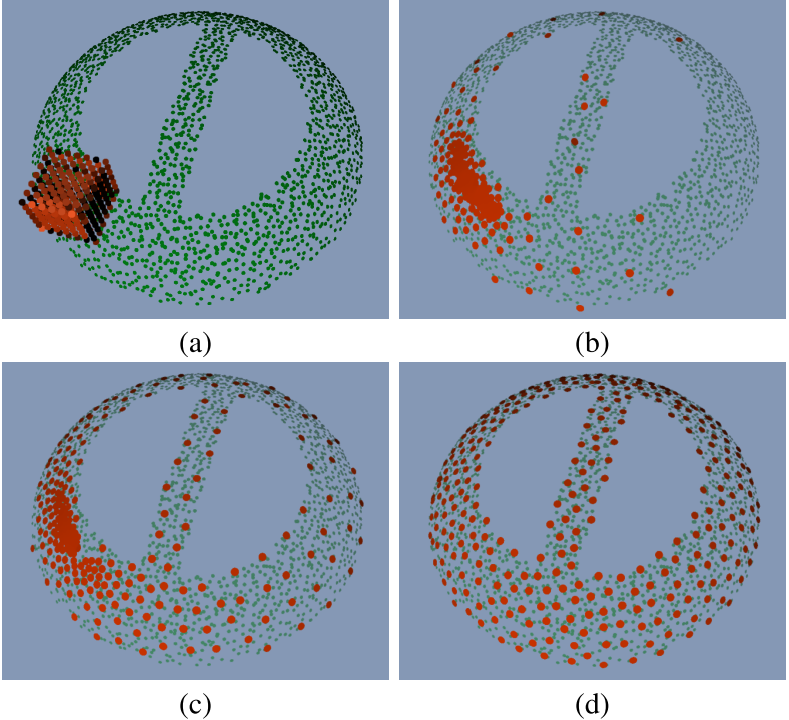
\includegraphics[width=2.0in]{images/L1median}
  \caption{Reconstruction by projection operation. (a). noisy point-set P(green) and an arbitrary point-set Q(red) that will be projected to P to approximate P. (b),(c) are two iterative projection results. (d) is the final projection.}
  \label{fig:L1 median}
\end{figure}

Reconstruction by a projection operator, as shown in Figure~\ref{fig:L1 median}, is to approximate the origin point set(green) by iteratively projecting an arbitrary point set(red) onto itself while removing the noises or outliers.
It has an important virtue: it defines a consistent geometry based on the data points, and provides constructive means to up-sample it.

$\ell_1$ median\cite{brown1983statistical,small1990survey}, closely related to projection operator, is a statistical tool applied globally to multivariate non-parametric point-samples in the presence of noises and outliers.
Briefly, it is a robust global center of an arbitrary set of points.
Given a data set $P=\{p_{j}\}_{j\in J}\subset \mathbb{R}^3$,
the $\ell_1$ median is defined as the point $q$ obtained by minimizing the sum of Euclidean distances to the data points

\small{
\begin{equation}
 \label{eq:L1median}
 q=\arg\min_{x}\left\{ \sum_{j\in J}^{}\|p_{j}-x\| \right\}
\end{equation}
}

\paragraph{(1)}

\cite{lipman2007parameterization} applies this tool locally to constitute a parameterization-free local projection operator(LOP).
Starting with an arbitrary initial point set $X^0=\{ x{_{i}^0}  \}_{i\in I}\subset \mathbb{R}^3$(typically $|X|\ll|P|$, $|\cdot|$ is the number of point set),
LOP computes the target point positions $X$ by performing a fixed-point iteration

\small{
\begin{equation}
 \label{eq:LOP1}
 X^{k+1}=\mathop{\argmin}_{X=\{x_{i}\}_{i\in I}}\{E_1(X^{k},P)+E_2(X^{k})\},\\
\end{equation}
}
\\
where,
\small{
\begin{equation}
 \label{eq:LOP2}
 \begin{split}
 & E_1(X^{k},P)=\sum_{i\in I}^{}\sum_{j\in J}^{}\|x_{i}-p_{j}\|\theta(\|x{_i^k}-p_{j}\|),\\
 & E_2(X^{k})=\sum_{i'\in I}^{}\lambda_{i'}\sum_{i\in I\setminus\{i'\}}^{} \eta(\|x_{i}-x{_{i'}^k}\|)\theta(\|x{_i^k}-x{_{i'}^k}\|).
 \end{split}
\end{equation}
}
\\
The term $E_1$ is in fact a $localized$ version of~(\ref{eq:L1median}) by using a fast-decaying weight function $\theta(r)=e^{-r^2/(h/4)^2}$ with the finite support radius $h$,
and thus it is just $E_1$ that drives the projected points $X$ to approximate the geometry of $P$.
The term $E_2$ keeps the distribution of the points $X$ fair by incorporating local repulsion forces.

To be convenient for the following works, now we give the expression of the solution. Let $\xi{_{ij}^k}=x{_i^k}-p_{j}$ and $\delta{_{ii'}^k}=x{_i^k}-x{_{i'}^k}$, solving~(\ref{eq:LOP1}), the projection for point $x{_i^{k+1}}$ is obtained as

\small{
\begin{equation}
 \label{eq:LOP3}
 x{_i^{k+1}}=F_1(x{_i^k},P)+F_2(x{_i^k},X{_i^{'}})
\end{equation}
}
\\
where,
\small{
\begin{equation}
 \label{eq:LOP4}
 \begin{split}
 & F_1(x{_i^k},P)=\sum_{j\in J}^{}p_{j}\frac{\alpha{_{ij}^k}}{\sum_{j\in J}^{}\alpha{_{ij}^k}},\\
 & F_2(x{_i^k},X{_i^{'}})=\mu\sum_{{i'}\in I\setminus\{i\}}^{}\delta{_{ii'}^k}\frac{\beta{_{ii'}^k}}{\sum_{{i'}\in I\setminus\{i\}}^{}\beta{_{ii'}^k}},\\
 & \alpha{_{ij}^k}=\frac{\theta(\|\xi{_{ij}^k}\|)}{\|\xi{_{ij}^k}\|},
   ~\beta{_{ii'}^k}=\frac{\theta(\|\delta{_{ii'}^k}\|)|\eta'(\|\delta{_{ii'}^k}\|)|}{\|\delta{_{ii'}^k}\|}.
 \end{split}
\end{equation}
}

Intuitively, LOP distributes the points by approximating their $\ell_1$ median to achieve robustness to outliers and data noises without any local orientation information nor a local manifold assumption.
But, also because of the use of the local density parameter $h$, it may not work well when the distribution of the input points is highly non-uniform and can fail to converge.

\paragraph{(2)}

Like\cite{lipman2007parameterization}, many consolidation methods try to obtain the resulted geometry object
without estimation of normals due to the unreliability resulting from the noisy data as oppose to the fact that
oriented normals at the points play a critical role in geometry reconstruction.

To achieve a better normal estimation that requires the sampling points to be uniformly distributed,
\cite{huang2009consolidation} incorporates locally adaptive density weights into LOP, resulting in a new consolidation technique WLOP, to address the non-uniform distribution problem while taking advantage of the success of LOP in denoising and outlier removal.

They define the weighted local densities for each point $p_{j}$ in $P$ and $x_{i}$ in $X$ during the $k$th iteration by $v_{j}=1+\sum_{j'\in J\setminus\{j\}}^{}\theta(\|p_{j}-p_{j'}\|)$ and $w{_i^k}=1+\sum_{i'\in I\setminus\{i\}}^{}\theta(\|\delta{_{ii'}^k}\|)$, the term $F_1$ and $F_2$ in~(\ref{eq:LOP4}) finally becomes

\small{
\begin{equation}
 \label{eq:WLOP}
 \begin{split}
 & F_1(x{_i^k},P)=\sum_{j\in J}^{}p_{j}\frac{\alpha{_{ij}^k}/v_{j}}{\sum_{j\in J}^{}(\alpha{_{ij}^k}/v_{j})}\\
 & F_2(x{_i^k},X{_i^{'}})=\mu\sum_{{i'}\in I\setminus\{i\}}^{}\delta{_{ii'}^k}\frac{w{_{i'}^k}\beta{_{ii'}^k}}{\sum_{{i'}\in I\setminus\{i\}}^{}(w{_{i'}^k}\beta{_{ii'}^k})},
 \end{split}
\end{equation}
}
\\
The weighted local density $v$ in $F_1$ relaxes the attraction of point clusters and
repulsion force in dense areas is strengthened by the local density $w$ in $F_2$.

Here, the obtained uniformly distributed point set can largely improve the reliability of normal initialization for a second normal estimation phase.
Practically, due to the high computational effort, it may not be a preferable choice to use this consolidation technique as a preprocessing method for surface reconstruction, even though some high quality surface can be reconstructed.


\paragraph{(3)}
In LOP/WLOP, the majority of the time is spent on the evaluation of the attractive forces from all points in $P$,
so \cite{preiner2014CPF} efficiently reduce the set $P$ of unordered input points to a much more compact mixture of Gaussians $\mathcal{M}=\{w_{s},\Theta_{s}\}$ that reflects the density distribution of the points.
That is, $\mathcal{M}$ defines a probability density function(pdf) as a weighted sum of $|\mathcal{M}|$ Gaussian components

\small{
\begin{equation}
 \label{eq:CLOP1}
 f(\mathbf{x}|\mathcal{M})=\sum_{s}^{}w_{s}g(\mathbf{x}|\Theta_{s}),
\end{equation}
}
\\
where the $\Theta_{s}=(\mu_{s},\sum_{s}^{})$ are the Gaussian parameters,
$w_{s}$ are their corresponding convex weights, and
$g$ denotes the $d$-variate Gaussian pdf.
%with $g(\mathbf{x}|\mu,\sum)=|2\pi\sum_{}^{}|^{-\frac{1}{2}}e^{-\frac{1}{2}(\mathbf{x}-\mu)^{T}\sum_{}^{-1}(\mathbf{x}-\mu)}$.

They define a $continuous$ $\mathcal{F}_1$ corresponding to $F_1$ in~(\ref{eq:LOP4}) by the convex sum over the internal attraction of each single Gaussian, with convex weights $w_s$ accounting for the Gaussian's relative point mass:

\small{
\begin{equation}
 \label{eq:CLOP2}
 \mathcal{F}_1(q,\mathcal{M})=\sum_{s}^{}w_s\int_{\mathbb{R}^3}^{}
 \frac{\mathbf{x}g(\mathbf{x}|\Theta_{s})\alpha(\mathbf{x})}
 {\sum_{s'}^{w_{s'}}\int_{\mathbb{R}^3}^{}g(\mathbf{x'}|\Theta_{s'})\alpha(x')d\mathbf{x}'}
 d\mathbf{x},
\end{equation}
}
\\
and the final \textbf{closed form} is expressed as
\small{
\begin{equation}
 \label{eq:CLOP3}
 \mathcal{F}_1(q,\mathcal{M})=\frac{\sum_{s}^{}\sum_{k}^{}\int_{\mathbb{R}^3}^{}\mathbf{x}\widehat{\Omega}_{sk}(\mathbf{x})d\mathbf{x}}
 {\sum_{s}^{}\sum_{k}^{}\int_{\mathbb{R}^3}^{}\widehat{\Omega}_{sk}(\mathbf{x})d\mathbf{x}}
 =\frac{\sum_{s,k}^{}w_{sk}\mu_{sk}}
 {\sum_{s,k}^{}w_{sk}}
\end{equation}
}
\\
changing the convex sum of 3D points $p_{j}$~(\ref{eq:LOP2}) into a convex combination of the product Gaussians' means $\mu_{sk}$ with weights $w_{sk}$.
Figure~\ref{fig:L1 median consolidation} shows the results of these three methods.

This continuous method is up to 7 times faster than an optimized GPU implementation of LOP/WLOP, and achieves interactive frame rates for moderately sized point clouds though it can not automatically get the best choice of the parameters for different point set.

\begin{figure}[ht]
  \centering
  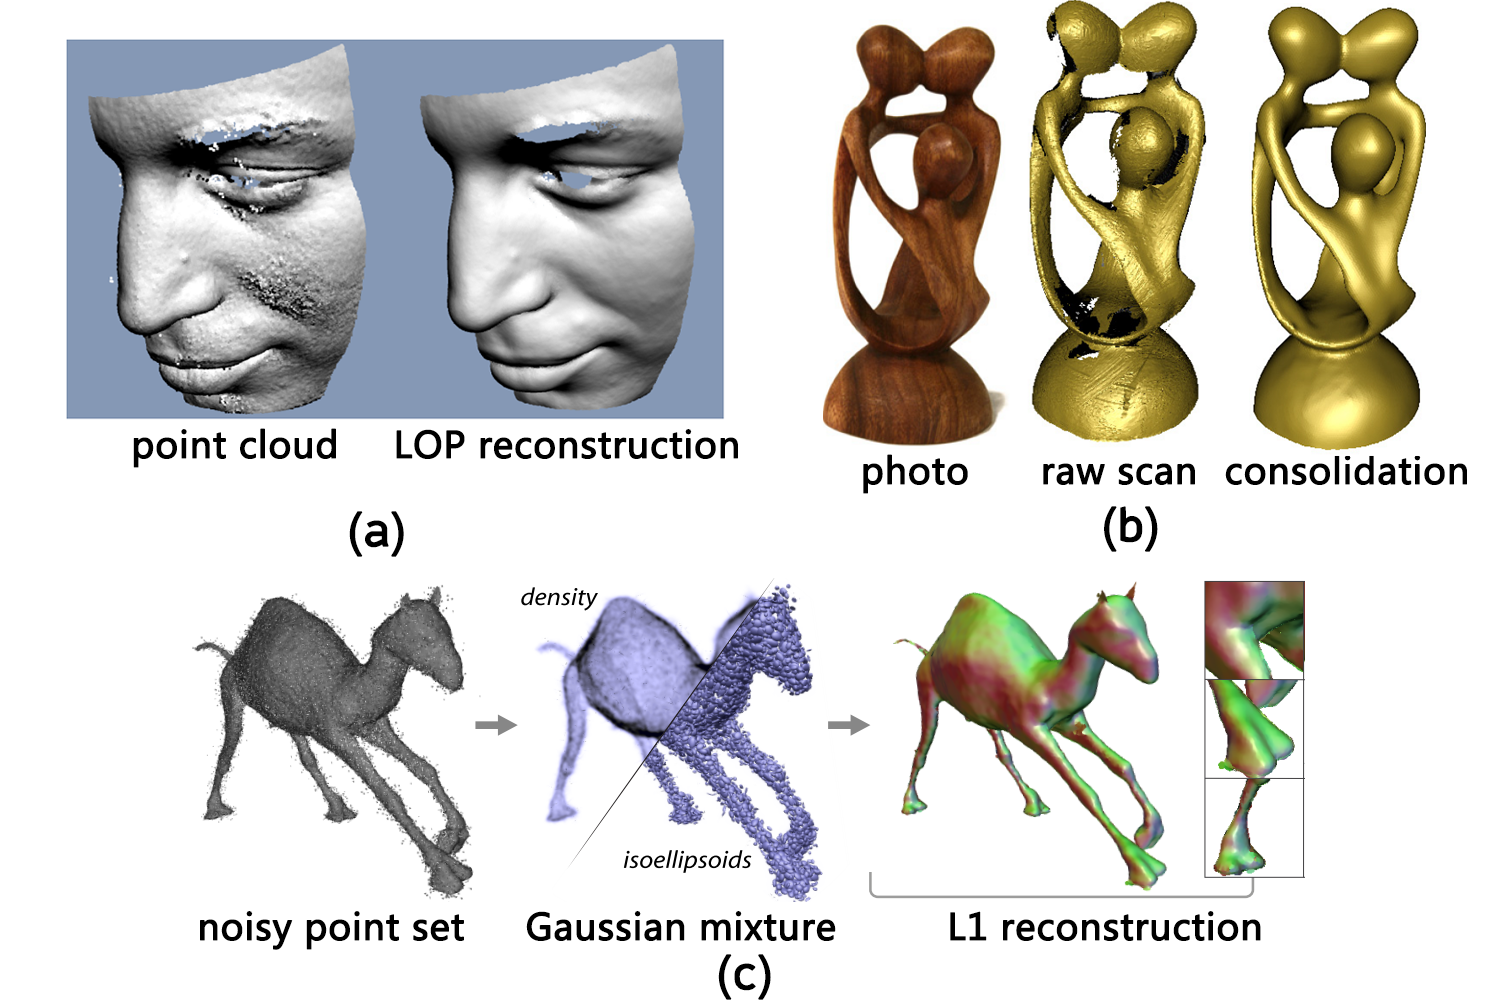
\includegraphics[width=2.5in]{images/reconstruction_L1}
  \caption{Sparse regularization: point cloud consolidation. (a): LOP\cite{lipman2007parameterization}. (b): WOLP\cite{huang2009consolidation}. (c): continuous WLOP\cite{preiner2014CPF}.}
  \label{fig:L1 median consolidation}
\end{figure}


\subsubsection{$\ell_1$ regression based}
Due to the robustness to noises and outliers of $\ell_1$ norm,
\cite{mustafa2014subdivision} develops an $\ell_1$ regression based subdivision algorithm for curve and surface fitting, 
where the size of target point cloud is largely more than that of origin data in contrast to the previous consolidation works.

For curve fitting, they try to find the best fit straight line $f(x)=\beta_1+\beta_2 x$ with observations$(x_r=r, f_r),r=-n+1,\cdots,n$.
The $\ell_1$ regression optimization is simply formulated as

\small{
\begin{equation}
 \label{eq:subdivision}
 \begin{split}
 &\beta_1, \beta_2 = \arg \min_{\beta_1,\beta_2\in\mathbb{R}}  \sum_{r=-n+1}^{n}  | f_r - (\beta_1 + \beta_2 r) |\\
 &~~~~~~~~=\arg \min_{\beta_1,\beta_2\in\mathbb{R}} F(\beta_1,\beta_2),
 \end{split}
\end{equation}
}
\\
because of the lack of differentiability, they regularize $F$ with a family of convex functional $F_{\delta}$, $\delta>0$,

\small{
\begin{equation}
 \label{eq:subdivision regularization}
 \begin{split}
 &F_{\delta}(\beta_1, \beta_2) = \sum_{r=-n+1}^{n}  h_{\delta}( f_r -\beta_1 - \beta_2 r),~\textrm{where}\\
 &h_{\delta}( f_r -\beta_1 - \beta_2 r) = [( f_r -\beta_1 - \beta_2 r)^2+\delta]^{1/2}
 \end{split}
\end{equation}
}
\\
then for a given $\delta$, the solution of (\ref{eq:subdivision}) is approximated by $\beta_{1,\delta}$ and $\beta_{2,\delta}$.
By substituting optimum $\beta_{1,\delta}$, $\beta_{2,\delta}$ into $f(x)$ and evaluating this function at 1/4 and 3/4,
the closed form of $\ell_1$ scheme for curve fitting is obtained.

With the closed form, $\ell_1$ scheme $D_{2n}$ firstly iteratively assigns weights to only $2n$ local initial points,
then gets the final fitting result(e.g.,Figure~\ref{fig:subdivision}) through subdivision rule for locations of vertices of the new mesh
and topological rule for size of added vertices and their connectivity.


\begin{figure}[ht]
  \centering
  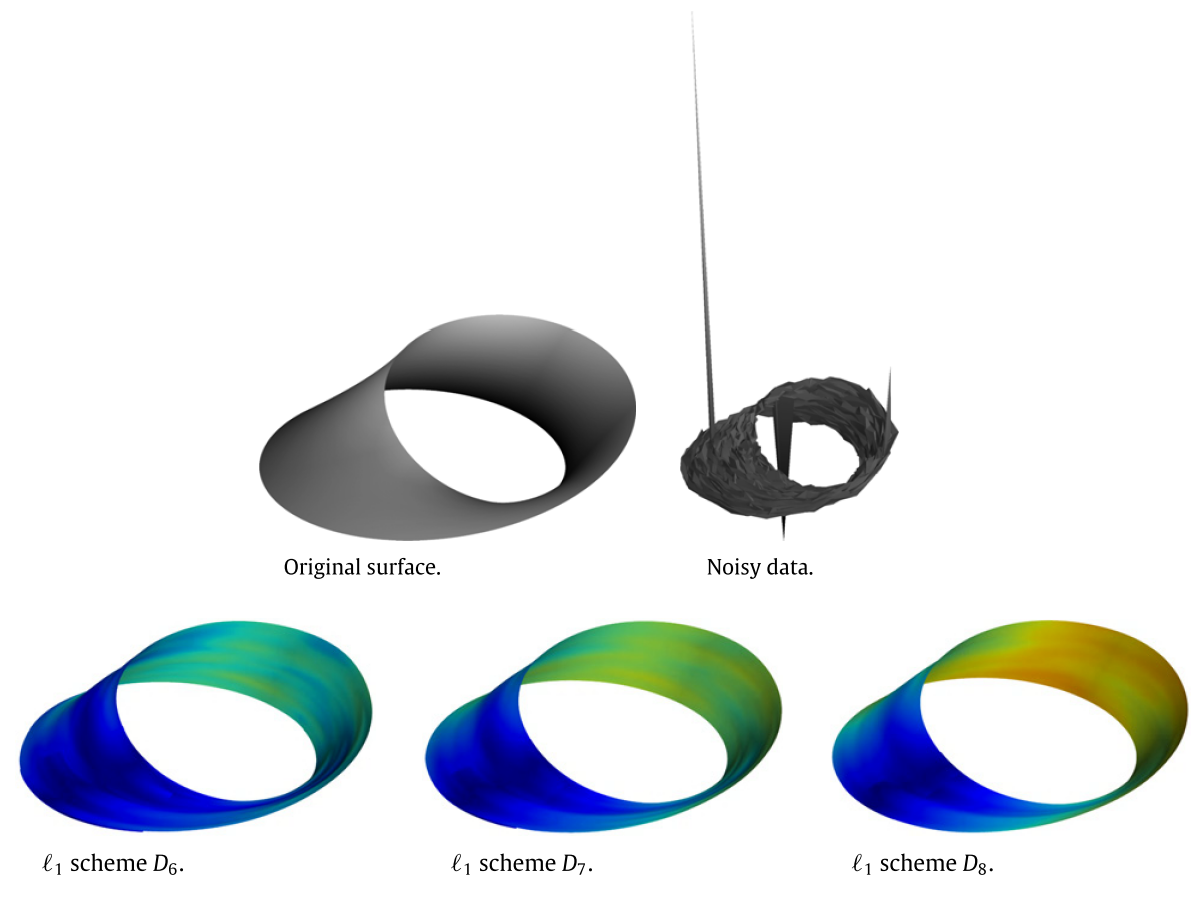
\includegraphics[width=2.5in]{images/subdivision}
  \caption{Sparse regularization: $\ell_1$ based subdivision\cite{mustafa2014subdivision}. Parametric surface reconstructed by $\ell_1$ scheme from highly noisy parametric data with outliers.}
  \label{fig:subdivision}
\end{figure}   % modeling & denoising
\subsection{Point Cloud Consolidation}
\label{subsec:Point Cloud Consolidation}


Nowadays, reconstructing the geometry of a shape from scanned data, also called point cloud consolidation, is a convenient and direct way to obtain 3D models.
It can be a preprocessing phase for some geometry problem, e.g., surface reconstruction whose result is a mesh object, with functionalities such as denoising, outlier removal, thinning, orientation, and redistribution of the input points.
However, current scanners are capable of producing large amount of raw, dense point sets with a variety of acquisition errors like noise, outliers, missing data(holes) or registration artifacts.
Then finding a robust reconstruction technique has always been an active researching area, and indeed there have been lots of works.
The works introduced in this section are all based on the $L_1$ median.

\subsubsection{$L_1$ median based}
\label{subsubsec:$L_1$ median based}

\begin{figure}[ht]
  \centering
  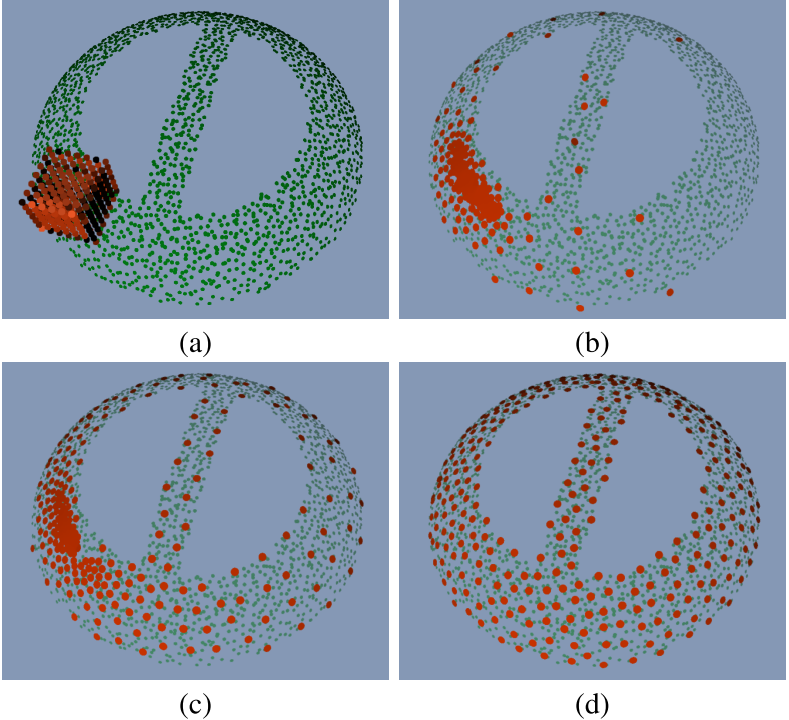
\includegraphics[width=2.5in]{images/L1median}
  \caption{Reconstruction by projection operation. (a). noisy point-set P(green) and an arbitrary point-set Q(red) that will be projected to P to approximate P. (b),(c) are two iterative projection results. (d) is the final projection.}
  \label{fig:L1 median}
\end{figure}

Reconstruction by a projection operator, as shown in Figure~\ref{fig:L1 median}, is to approximate the origin point-set(green) by iteratively projecting an arbitrary point-set(red) onto itself while removing the noises or outliers.
It has an important virtue: it defines a consistent geometry based on the data points, and provides constructive means to up-sample it.

A new projection operator is introduced via a certain fixed-point iteration where the approximated geometry consists of its stationary points,
and it is closely related to the $L_1$ median\cite{brown1983statistical,small1990survey} which is a statistical tool that applied globally to multivariate non-parametric point-samples in the presence of noise and outliers.
Briefly, it is a robust global center of an arbitrary set of points. Mathematically, given a data set $P=\{p_{j}\}_{j\in J}\subset \mathbb{R}^3$, the $L_1$ median is defined as the point $q$ obtained by minimizing the sum of Euclidean distances to the data points

\small{
\begin{equation}
 \label{eq:L1median}
 q=\arg\min_{x}\left\{ \sum_{j\in J}^{}\|p_{j}-x\| \right\}
\end{equation}
}

\paragraph{(1)}

\cite{lipman2007parameterization} applies this tool locally to constitute a robust reconstruction mechanism called parameterization-free local projection operator(LOP).
Starting with an arbitrary initial point-set $X^{(0)}=\{{x_{i}}^{(0)}\}_{i\in I}\subset \mathbb{R}^3$(typically $|X|\ll|P|$, $|\cdot|$ is the number of point-set),
LOP computes the target point positions $X$ by performing a fixed-point iteration

\small{
\begin{equation}
 \label{eq:LOP1}
 X^{k+1}=\mathop{\argmin}_{X=\{x_{i}\}_{i\in I}}\{E_1(X^{k},P)+E_2(X^{k})\},\\
\end{equation}
}
\\
where,
\small{
\begin{equation}
 \label{eq:LOP2}
 \begin{split}
 & E_1(X^{k},P)=\sum_{i\in I}^{}\sum_{j\in J}^{}\|x_{i}-p_{j}\|\theta(\|x{_i^k}-p_{j}\|),\\
 & E_2(X^{k})=\sum_{i'\in I}^{}\lambda_{i'}\sum_{i\in I\setminus\{i'\}}^{} \eta(\|x_{i}-x{_{i'}^k}\|)\theta(\|x{_i^k}-x{_{i'}^k}\|).
 \end{split}
\end{equation}
}
\\
The term $E_1$ is in fact a localized version of~(\ref{eq:L1median}) by using a fast-decaying weight function $\theta(r)=e^{-r^2/(h/4)^2}$ with the finite support radius $h$,
and thus it is just $E_1$ that drives the projected points $X$ to approximate the geometry of $P$.
The term $E_2$ keeps the distribution of the points $X$ fair by incorporating local repulsion forces.

Let $\xi{_{ij}^k}=x{_i^k}-p_{j}$ and $\delta{_{ii'}^k}=x{_i^k}-x{_{i'}^k}$, solving~(\ref{eq:LOP1}), the projection for point $x{_i^{k+1}}$ is obtained as

\small{
\begin{equation}
 \label{eq:LOP3}
 x{_i^{k+1}}=F_1(x{_i^k},P)+F_2(x{_i^k},X{_i^{'}})
\end{equation}
}
\\
where,
\small{
\begin{equation}
 \label{eq:LOP4}
 \begin{split}
 & F_1(x{_i^k},P)=\sum_{j\in J}^{}p_{j}\frac{\alpha{_{ij}^k}}{\sum_{j\in J}^{}\alpha{_{ij}^k}},\\
 & F_2(x{_i^k},X{_i^{'}})=\mu\sum_{{i'}\in I\setminus\{i\}}^{}\delta{_{ii'}^k}\frac{\beta{_{ii'}^k}}{\sum_{{i'}\in I\setminus\{i\}}^{}\beta{_{ii'}^k}},\\
 & \alpha{_{ij}^k}=\frac{\theta(\|\xi{_{ij}^k}\|)}{\|\xi{_{ij}^k}\|},
   ~\beta{_{ii'}^k}=\frac{\theta(\|\delta{_{ii'}^k}\|)|\eta'(\|\delta{_{ii'}^k}\|)|}{\|\delta{_{ii'}^k}\|}.
 \end{split}
\end{equation}
}

Intuitively, LOP distributes the points by approximating their $L_1$ median to achieve robustness to outliers and data noises without any local orientation information nor a local manifold assumption.
However, also because of the use of the local density parameter $h$, it may not work well when the distribution of the input points is highly non-uniform and can fail to converge.

\paragraph{(2)}

Like\cite{lipman2007parameterization}, many surface reconstruction methods try to obtain the resulted mesh without estimation of normals due to the unreliability because of the noisy data.
In fact, oriented normals at the points play a critical role in surface reconstruction and the estimation of normals requires the sampling points to be uniformly distributed.
\cite{huang2009consolidation} proposes a new consolidation technique whose central task is normal estimation.

To take advantage of the success of LOP in denoising and outlier removal, and simultaneously address the non-uniform distribution problem, they incorporate locally adaptive density weights into LOP, resulting in WLOP, they define the weighted local densities for each point $p_{j}$ in P and $x_{i}$ in X during the $k$th iteration by $v_{j}=1+\sum_{j'\in J\setminus\{j\}}^{}\theta(\|p_{j}-p_{j'}\|)$ and $w{_i^k}=1+\sum_{i'\in I\setminus\{i\}}^{}\theta(\|\delta{_{ii'}^k}\|)$, the term $F_1$ and $F_2$ in () finally becomes

\small{
\begin{equation}
 \label{eq:WLOP}
 \begin{split}
 & F_1(x{_i^k},P)=\sum_{j\in J}^{}p_{j}\frac{\alpha{_{ij}^k}/v_{j}}{\sum_{j\in J}^{}(\alpha{_{ij}^k}/v_{j})}\\
 & F_2(x{_i^k},X{_i^{'}})=\mu\sum_{{i'}\in I\setminus\{i\}}^{}\delta{_{ii'}^k}\frac{w{_{i'}^k}\beta{_{ii'}^k}}{\sum_{{i'}\in I\setminus\{i\}}^{}(w{_{i'}^k}\beta{_{ii'}^k})},
 \end{split}
\end{equation}
}
\\
The weighted local density $v$ in $F_1$ relaxes the attraction of point clusters and repulsion force in dense areas is strengthened by the local density $w$ in $F_2$.

So far, we actually have obtained a reconstructed point set which will then be used to improve the reliability of normal initialization that will be used in a second normal estimation phase.
However, considering the high computational effort, it may not be a preferable choice using this consolidation technique as a preprocessing method for surface reconstruction even though some high quality surface can be reconstructed.


\paragraph{(3)}
In LOP/WLOP, the majority of the time is spent on the evaluation of the attractive forces from all points in $P$,
so \cite{preiner2014CPF} efficiently reduce the set $P$ of unordered input points to a much more compact mixture of Gaussians $\mathcal{M}=\{w_{s},\Theta_{s}\}$ that reflects the density distribution of the points.
That is, $\mathcal{M}$ defines a probability density function(pdf) as a weighted sum of $|\mathcal{M}|$ Gaussian components

\small{
\begin{equation}
 \label{eq:CLOP1}
 f(\mathbf{x}|\mathcal{M})=\sum_{s}^{}w_{s}g(\mathbf{x}|\Theta_{s}),
\end{equation}
}
\\
where the $\Theta_{s}=(\mu_{s},\sum_{s}^{})$ are the Gaussian parameters, $w_{s}$ their corresponding convex weights, and $g$ denotes the $d$-variate Gaussian pdf with $g(\mathbf{x}|\mu,\sum)=|2\pi\sum_{}^{}|^{-\frac{1}{2}}e^{-\frac{1}{2}(\mathbf{x}-\mu)^{T}\sum_{}^{-1}(\mathbf{x}-\mu)}$.

They define a $continuous$ $\mathcal{F}_1$ corresponding to $F_1$ in~(\ref{eq:LOP4}) by the convex sum over the internal attraction of each single Gaussian, with convex weights $w_s$ accounting for the Gaussian's relative point mass:

\small{
\begin{equation}
 \label{eq:CLOP2}
 \mathcal{F}(q,\mathcal{M})=\sum_{s}^{}w_s\int_{\mathbb{R}^3}^{}
 \frac{\mathbf{x}g(\mathbf{x}|\Theta_{s})\alpha(\mathbf{x})}
 {\sum_{s'}^{w_{s'}}\int_{\mathbb{R}^3}^{}g(\mathbf{x'}|\Theta_{s'})\alpha(x')d\mathbf{x}'}
 d\mathbf{x},
\end{equation}
}
\\
and the final \textbf{closed form} is expressed as
\small{
\begin{equation}
 \label{eq:CLOP3}
 \mathcal{F}(q,\mathcal{M})=\frac{\sum_{s}^{}\sum_{k}^{}\int_{\mathbb{R}^3}^{}\mathbf{x}\widehat{\Omega}_{sk}(\mathbf{x})d\mathbf{x}}
 {\sum_{s}^{}\sum_{k}^{}\int_{\mathbb{R}^3}^{}\widehat{\Omega}_{sk}(\mathbf{x})d\mathbf{x}}
 =\frac{\sum_{s,k}^{}w_{sk}\mu_{sk}}
 {\sum_{s,k}^{}w_{sk}},
\end{equation}
}
\\
where in the same way that~(\ref{eq:LOP2}) is convex of 3D points $p_{j}$, now becomes a convex combination of the product Gaussians' means $\mu_{sk}$ with weights $w_{sk}$.

This method is up to 7 times faster than an optimized GPU implementation of LOP/WLOP, and achieves interactive frame rates for moderately sized point clouds though it can not automatically get the best choice of the parameters for different point set.

\vspace{10pt}
Figure~\ref{fig:L1 median consolidation} shows the results of these three methods. In summary, many robust point cloud consolidation or surface reconstruction techniques have been developed to deal with a variety of acquisition errors like noise, outliers, missing data(holes) or registration artifacts.
Most of the $l_1$ techniques are typically too expensive to achieve interactive reconstruction times for at least moderately sized point sets, even for parallel implementations,
and are designed for quality rather than performance due to their nature. So the performance problem is still challenging and worth researching. 

\begin{figure}[ht]
  \centering
  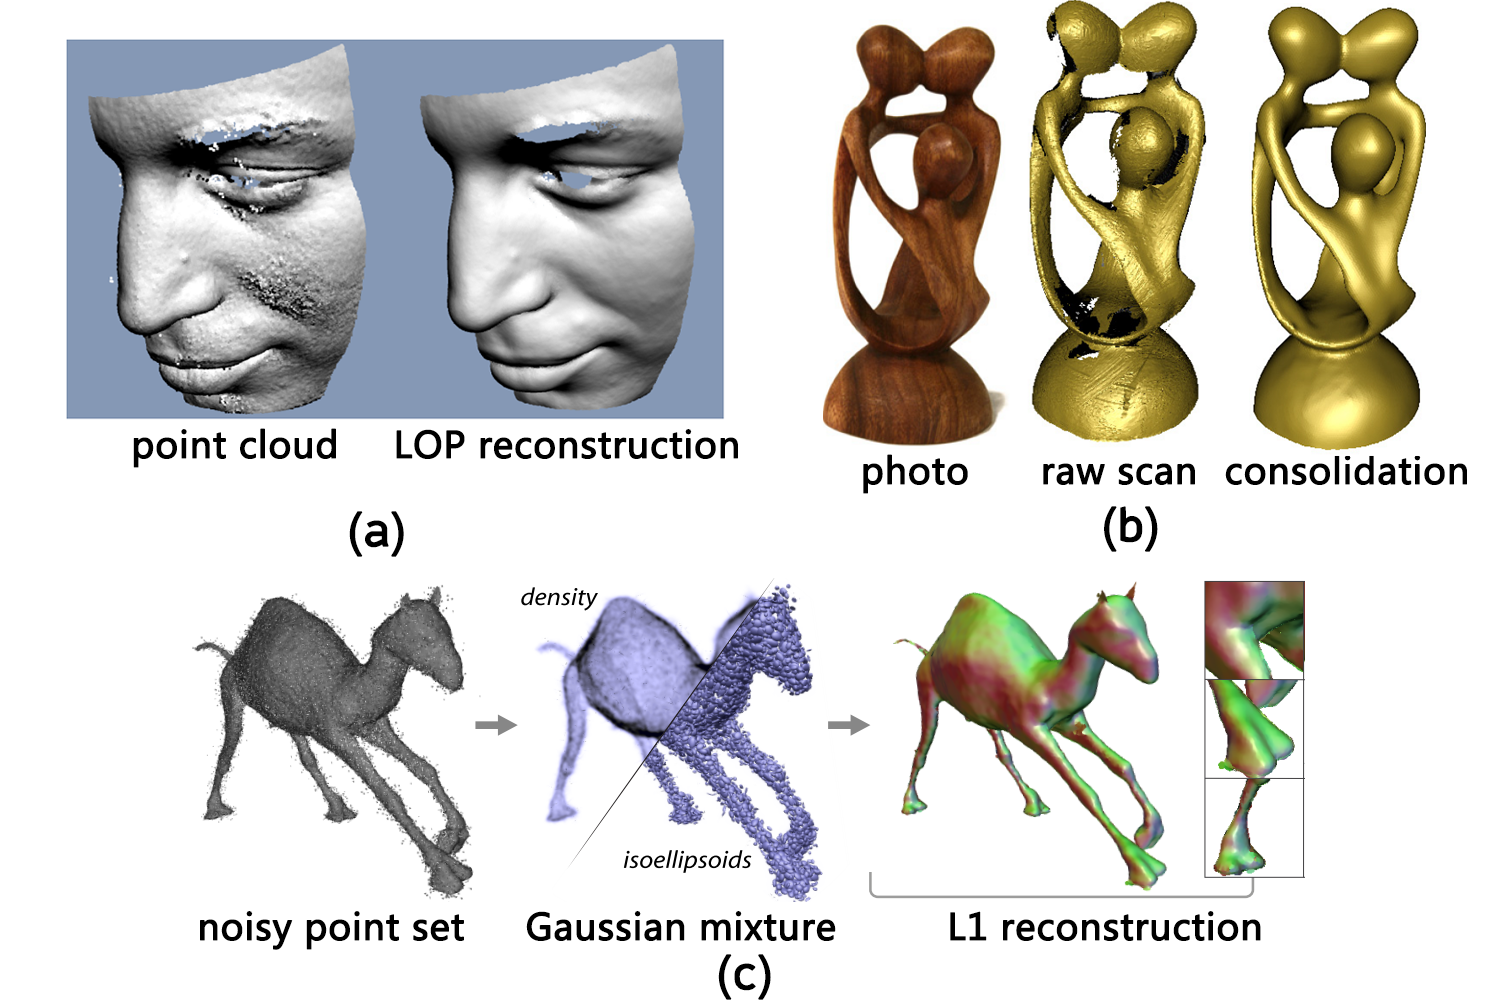
\includegraphics[width=3in]{images/reconstruction_L1}
  \caption{Sparse regularization: point cloud consolidation. (a): LOP\cite{lipman2007parameterization}. (b): WOLP\cite{huang2009consolidation}. (c): continuous WLOP\cite{preiner2014CPF}.}
  \label{fig:L1 median consolidation}
\end{figure}  % reconstruction based on L_1 median and TV

\subsection{Shape Matching}

Here, we give shape matching a more extensive definition: finding the correspondence(point-wise, pair-wise) between two rigid or non-rigid deformable geometric data sets.

\subsubsection{Rigid registration} Rigid registration is a fundamental task in computer graphics and geometry processing. It aims at finding a suitable set of corresponding points on source and target point set. The $Iterative~Closest~Point$(ICP) addresses this problem by assuming the input data to be in coarse alignment. Under this assumption, a set of correspondences can be obtained by querying closest points on the target geometry. Given two surfaces $\mathcal{X}$, $\mathcal{Y}$, it is formulated as

\small{
\begin{equation}
 \label{eq:ICP}
 \mathop{\argmin}_{\mathbf{R},\mathbf{t}}\int_{\mathcal{X}}^{}\varphi(\mathbf{Rx}+\mathbf{t},\mathcal{Y})d\mathbf{x}+I_{\mathcal{SO}(k)}(\mathbf{R})
\end{equation}
}
\\
where $\mathbf{R}$ is a rotation matrix, $\mathbf{t}$ is a translation vector, $\mathbf{x}$ is a point on the source geometry. The quality of a registration is evaluated by the metric $\varphi(\mathbf{x},\mathbf{y})=\|\mathbf{x}-\mathbf{y}\|{_2^2}$, i.e., classical ICP is in a least-square sense which would fail with outliers.

Now that sparse regularization methods excels in processing data set with noises or outliers, \cite{bouaziz2013sparse} tries to formulate the local alignment problem as recovering rigid transformation that minimizes the number of zero distances between two correspondences. Since \cite{chartrand2007exact} shows that $l_{p}$ norms with $p<1$ outperform the $l_1$ norm in inducing sparsity and \cite{elad2010sparse} also illustrates the tendency of $l_{p}$($0<p<1$)norms to drive results to become sparse. \cite{bouaziz2013sparse} adopts $l_{p}$($0\le p\le1$) norm based sparse regularizer to obtain an heuristic-free, robust rigid registration algorithm by modifying

\small{
\begin{equation}
 \label{eq:permutedsparse}
 \varphi(\mathbf{x},\mathbf{y})=\|\mathbf{x}-\mathbf{y}\|{_2^{p}}
\end{equation}
}

Figure...is the registration results of sparse ICP under different values of $p$ among which it can be found that $0<p<1$ reduces better results, but the value of $p$ is selected according to the experiments to offer a trade-off between performance and robustness which may make the sparse ICP unpractical.

\begin{figure}[ht]
  \centering
  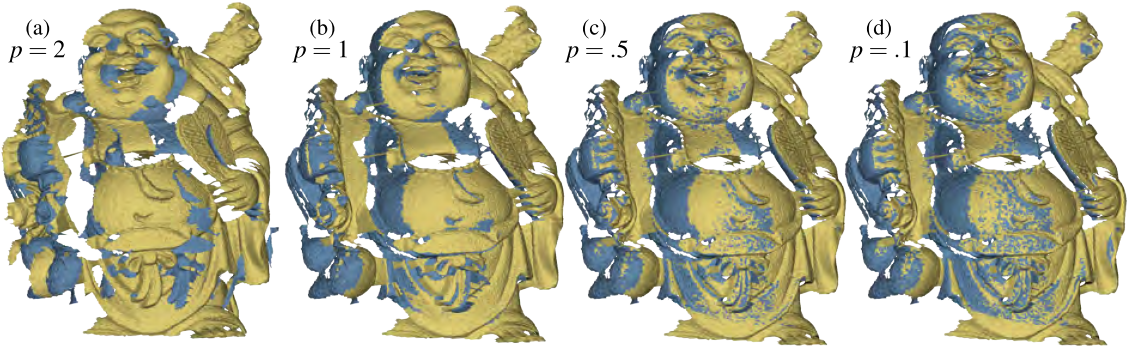
\includegraphics[width=3in]{images/sparseICP}
  \caption{Sparse regularization: rigid registration results using sparse ICP\cite{chartrand2007exact} under different $l_{p}$ norms.}
\end{figure}

\subsubsection{Non-rigid shape matching}
Matching of deformable shapes is a notoriously difficult problem playing an important role in many application, non-rigid matching typically uses point-wise representation of correspondence, which results in the number of degrees of freedom growing exponentially with the number of matched points.

Recently, \cite{ovsjanikov2012functional} introduces a functional representation for correspondences which are modeled as the correspondences between functions on two shapes rather than points.
Briefly, let $X$ and $Y$ be two shapes equipped with bases $\{\phi_{i}\}_{i\ge1}$ and $\{\psi_{j}\}_{j\ge1}$ respectively, any real function $f: X\to \mathbb{R}$ and $g=T(f): Y\to \mathbb{R}$ can be represented as $f=\sum_{i\ge1}^{}a_{i}\phi_{i}$ and $g=\sum_{j\ge1}^{}b_{j}\psi_{j}$.
Taking discretized functions $\phi_{i}$ and $\psi_{j}$ as the columns of bases matrices $\Phi$ and $\Psi$, the functions vectors...$\mathbf{b^{T}}=\mathbf{a^{T}C}$. Thus, the matrix $\mathbf{C}$ fully encodes the linear map $T$ between the functional spaces.
In case the shapes $X$ and $Y$ are isometric and the corresponding Laplace-Beltrami operators have simple spectra, the harmonic bases(Laplacian eigenfunctions) have a compatible behavior, $\psi_{i}=T(\phi_{i})$ such that $c_{ij}=\delta_{ij}$.
Choosing the discretized eigenfunctions of the Laplace-Beltrami operator as $\Phi$ and $\Psi$ causes every low-distortion correspondence being represented by a nearly diagonal, and therefore very sparse matrix $C$.

Based on the above theory, \cite{pokrass2013sparse} firstly gets two collections of similar functions $\{f_{i}:X\to \mathbb{R}\}$ and $\{g_{j}:Y\to \mathbb{R}\}$ using some region detection process like\cite{litman2011diffusion}. \parpic[r]{\label{fig:regionmatching}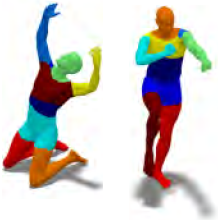
\includegraphics[width=0.4\linewidth]{images/matching_function}}As shown in the right figure, different colors represent different functions and the correspondence of these two collections of functions is unknown, i.e., we do not know to which $g_{j}$ in $Y$ a $f_{i}$ in $X$ corresponds.
\cite{pokrass2013sparse} adopts an unknown permutation matrix $\mathbf{\Pi}$ to express this ordering. Finally, the robust permuted sparse coding is formulated as following

\small{
\begin{equation}
 \label{eq:permutedsparse}
 \min_{\mathbf{C},\mathbf{O},\mathbf{\Pi}}\frac{1}{2}\|\mathbf{\Pi}\mathbf{B}-\mathbf{AC}-\mathbf{O}\|{_{F}^2}+\lambda\|\mathbf{W}\odot\mathbf{C}\|_1+\mu\|\mathbf{O}\|_{2,1}
\end{equation}
}
\\
where $\mathbf{W}$ is assigned with larger weights in off-diagonal part and small weights in diagonal part to promote diagonal solutions, $\|\mathbf{O}\|_{2,1}$ promotes row-wise sparsity allowing to absorb the errors in the data term corresponding to the rows of $\mathbf{A}$ having no corresponding rows in $\mathbf{B}$.
Figure...This method relies on the region detection technique and assumption: near-isometric shapes.

\begin{figure}[ht]
  \centering
  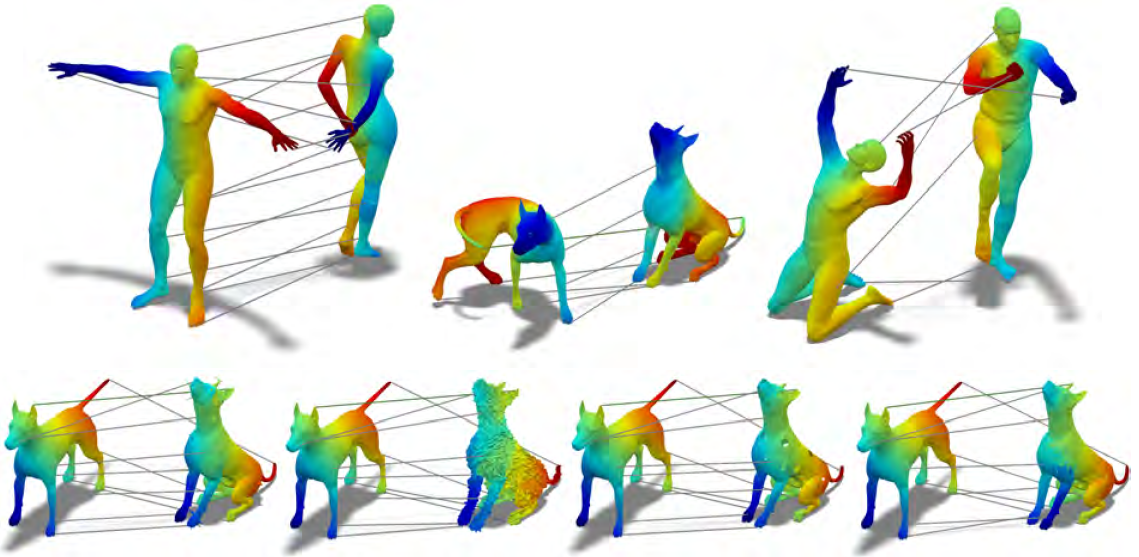
\includegraphics[width=3in]{images/matching_L1}
  \caption{Sparse regularization: non-rigid shape matching \cite{wang2014decoupling}. First row: point-to-point correspondences between different non-isometric shapes. Second row: point-to-point correspondence between SHREC shapes undergoing nearly isometric deformations and noise.}
\end{figure}


\subsubsection{Co-segmentation}
Co-segmentation aims to consistently segment a group of shapes and obtain the correspondence between resulted segments simultaneously. As (b) in figure...shows, corresponding parts are labeled in the same colors.
To be more intuitive and efficient, \cite{hu2012co} processes co-segmentation on patch-level instead of face-level like many other works.

So they firstly over-segment all the models((a) in figure) followed by calculating their feature vectors using some feature descriptors.
For example, figure... shows the colormaps of average geodesic distance(AGD) features of two tables with over-segmented patches, and actually there are $H=5$ feature descriptors.
They define the feature vector as a histogram of the feature measurement on the triangles of that patch.
Then it is obvious that two corresponding patches have similar distributions, which means their feature vectors lie in a common subspace generated by standard basis corresponding to these nonzero entries.
Based on this observation, they regard co-segmentation as a subspace clustering problem since the final segments are all clustering of patches.

\begin{figure}[ht]
  \centering
  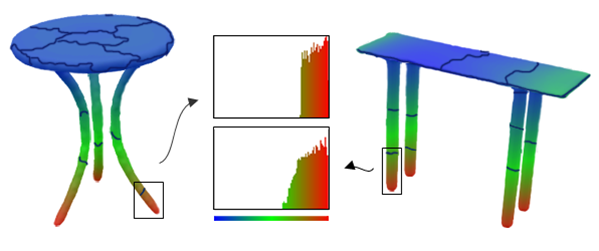
\includegraphics[width=3in]{images/co-segmentationAGD}
  \caption{Sparse regularization: co-segmentation\cite{hu2012co}. Colormaps of AGD features of two tables with over-segmented patches. The AGD feature vectors of the two patches(marked in rectangles) from each table's leg have similar distribution, as shown in histograms in the middle. It can be seen that these two feature vectors lie in the common subspace generated by standard basis corresponding to the nonzero entries.}
\end{figure}


Since that each data point(here is the feature vector) in a union of linear subspaces can always be represented as a linear combination of the points belonging to the same linear subspace and thus the combination could be sparse if the point is written as a linear combination of all other points. Following\cite{elhamifar2009sparse,wang2011efficient}, finding the sparse combination matrix for the single-feature co-segmentation is formulated as

\small{
\begin{equation}
 \label{eq:SSC}
 \begin{split}
 &\min_{W_{h}}\|X_{h}W_{h}-X_{h}\|{_{F}^2}+\lambda\|W_{h}^{T}W_{h}\|_{1,1} \\
 &s.t.~W_{h}\ge0,~\textrm{diag}(W_{h})=0
 \end{split}
\end{equation}
}
\\
where $h$ corresponds to the $h$-th feature descriptor,
the feature matrix $X_{h}=[x_{h1},x_{h2},\cdots,x_{hN}]$ is constructed with $x_{hi}$ which is the feature vector of the $i$-th patch($i=1,2,\cdots,N$).
$\|W_{h}^{T}W_{h}\|_{1,1}$ is seen as a penalty item in the optimization, which favors the sparsity of the optimal solution $\overline{W_{h}}$ of which each entry measures the linear correlation between two points in the meshes.
After defining the affinity matrix $S=(s_{ij})$ as $s_{ij}=|\overline{w_{h}}_{ij}|+|\overline{w_{h}}_{ji}|$, the NCut method\cite{shi2000normalized} is applied to get the co-segmentation results.

However, single one feature is not enough for co-segmenting different categories of models.
Taking two following things into account:
finding the most similar patch pairs considering selected features and corresponding patches need not be similar in these features,
\cite{hu2012co} adds the consistent multi-feature penalty to ensure the co-segmentation results consistent with different feature spaces by combing $H$ feature descriptors

\small{
\begin{equation}
 \label{eq:SSC}
 \begin{split}
 &\min_{W_{1},\cdots,W_{H}}\sum_{h=1}^{H}\mathcal{F}(W_{h})+\mathcal{P}_{cons}(W_1,W_2,\cdots,W_H)\\
 &s.t.~W_{h}\ge0,~\textrm{diag}(W_{h})=0,h=1,2,\cdots,H.
 \end{split}
\end{equation}
}
\\
where $\mathcal{P}_{cons}$ is the penalty on the matrices $W_1,W_2,\cdots,W_H$

\small{
\begin{equation}
 \label{eq:SSC}
 \mathcal{P}_{cons}(W_1,W_2,\cdots,W_H)=\alpha\|W\|_{2,1}+\beta\|W\|_{1,1}\\
\end{equation}
}
\\
here the $H\times N^2$ matrix $W$ is formed by concatenating $W_1,W_2,\cdots,W_H$(each matrix in one row) together:

\small{
\begin{equation}
 \label{eq:edgecotanoperator}
 W = {\left[ \begin{array}{cccc}
 (W_1)_{11} & (W_1)_{12} & \cdots & (W_1)_{N^2}\\
 (W_2)_{11} & (W_2)_{12} & \cdots & (W_2)_{N^2}\\
 \vdots & \vdots & \ddots & \vdots\\
 (W_{H})_{11} & (W_{H})_{12} & \cdots & (W_{H})_{N^2}
 \end{array}
 \right]}
\end{equation}
}
\\
the $\ell_{2,1}$ penalty on $W$ induces column sparsity of $W$ such that most columns of $W$ are shrunken to be entirely zero, which means that the corresponding pairs of patches will likely not be in the same cluster.
The $\ell_{1,1}$ penalty on $W$ induces the sparsity within each column of $W$.
This means that for each non-zero column, that is for each similar patch pair, only a subset of features are actually used to measure their similarity.
Hence this term enables the prominent features to pop up and guarantees the sparsity-consistency of the matrices $W_1,W_2,\cdots,W_H$.

Notice that without $\mathcal{P}_{cons}$, the formulation () will reduce to a naive solution which is exactly the same as applying subspace clustering to each feature matrix $X_{h}$ independently.

\begin{figure}[ht]
  \centering
  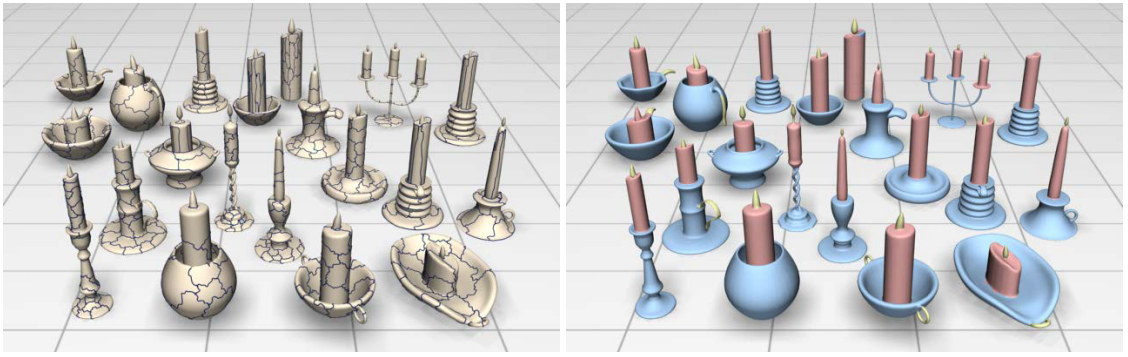
\includegraphics[width=3in]{images/co-segmentation}
  \caption{Sparse regularization: co-segmentation\cite{hu2012co}. Left shows the over segmented patches that will be clustered to get the co-segmentation result.}
\end{figure}



\subsection{Barycentric coordinates}
$\mathbf{Barycentric~coordinates}$ provide a simple and convenient way of interpolating values from a set of control points over the interior of a domain, using weighted combinations of values associated with different control points. Current barycentric coordinates typically are of global nature, meaning that the interpolated value depends on many, potentially $all$, control points. Besides the lack of locality and scalability, the interpolation is computationally expensive since it involves a weighted sum of all control points for each interior vertex. Thus, barycentric coordinates with locality provide benefit in terms of storage requirements as well as computational cost. $\mathbf{Juyong~Zhang}$ introduces a novel method to derive $local~barycentric~coordinates$(LBC), which depend only on a small number of control points. LBC are computed by minimizing a target functional based on total variation, subject to a set of constraints that ensure desired properties such as locality, linearity, non-negativity, and smoothness. LBC induce lower computational cost for applications such as cage-based deformation(Figure...), since each point on the target shape is only determined by a small number of control points.

\begin{figure}[ht]
  \centering
  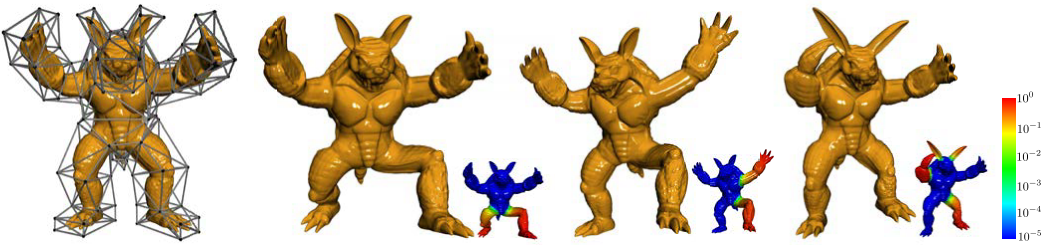
\includegraphics[width=3in]{images/LBC_L1}
  \caption{Sparse regularization: local barycentric coordinates\cite{}. Using LBC for 3D cage-based manipulation allows for local, smooth and shape-aware deformations. Only parts near the manipulated control points are deformed, as indicated by the color-coding.}
\end{figure}


\subsection{Skeleton extraction}
In section..., we have introduced much information about $L_1$ median and its success in point cloud consolidation.
Except for reducing 2D surface that approximate origin point-set, \cite{huang2013l1} observed that adapting $L_1$ medians $locally$ to a point set representing a geometric shape also gives rise to a $one-dimensional$ structure which can be seen as a localized center of the shape, i.e., a medial curve skeleton that can be used for shape abstraction and consequently an effective tool for shape analysis and manipulation\cite{cornea2007curve}.
Without building any point connectivity or estimating point normals, they directly project point samples onto their local centers as $l_1$ medians with growing neighborhood and push the projected samples via conditional regularization to obtain a uniform distribution of samples along skeleton branches.

It is intuitively a modification of LOP by modifying the repulsion term $E_2$ in () and proposing a different weighted density parameter that can also be named WLOP\cite{huang2009consolidation}. Re-centering. Figure... shows an example.

\begin{figure}[ht]
  \centering
  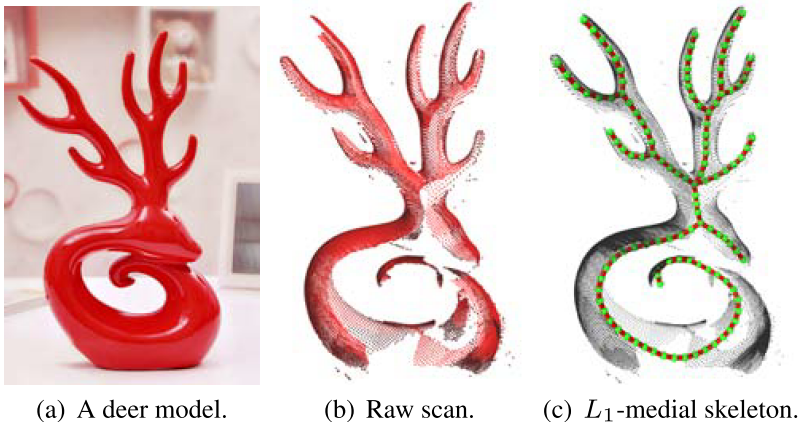
\includegraphics[width=3in]{images/skeleton_L1}
  \caption{Sparse regularization: skeleton extraction\cite{huang2013l1}. Given an unorganized, unoriented, and incomplete raw scan with noise and outliers(b), a complete and quality curve skeleton is extracted(c).}
\end{figure}


\subsection{Constrained modeling} Constrained modeling is an important tool for the construction and modification of 3D geometric models. Especially in the case of modeling man-made structure like architecture or machine parts, geometric constraints are able to create and preserve ubiquitous alignment properties like element parallelism, conllinearity, fixed angles and distances, or symmetry relations. Generally, analyzing and solving constraint systems usually fail to meet two main challenges of an interactive 3D modeling system: for each atomic editing operation, it is crucial to adjust as few auxiliary vertices as possible in order to not destroy the user's earlier editing effort; the whole constraint resolution pipeline is required to run in real-time to enable a fluent, interactive workflow.

To address both issues, \cite{habbecke2012linear} presents a novel interactive constrained modeling with a well-defined strategy that, for an atomic editing operation, computes $as~small~as~possible$ model updates in terms of the total number of adjusted vertices.

Mathematically, a model instance $\mathbf{X}_0$, whose elements are the vertex positions, satisfies all constraints denoted by $\mathbf{c}(\mathbf{X}_0)=\mathbf{0}$ which is a vector-valued function. Then for a given editing displacement $\mathbf{d}$ corresponding to one user editing operation, the central goal is to find a correction displacement $\mathbf{d'}$  such that $\mathbf{c}(\mathbf{X}_0+\mathbf{d}+\mathbf{d'})=\mathbf{0}$, where the zero elements of $\mathbf{d'}$ and $\mathbf{d}$ are disjoint and $\mathbf{d'}$ should be as sparse as possible.

If the space of possible movements of each vertex $\mathbf{x}_{i}$ is represented with a basis $\{\mathbf{b}_{i,1},\mathbf{b}_{i,1},\mathbf{b}_{i,3}\}$, $\mathbf{b}_{i,k} \in \mathbb{R}^3$, after extending the 3-dimensional basis vectors to vectors $\mathbf{B}_{i,k}:=(0,...,0,\mathbf{b}{_{i,k}^{T}},0,...,0) \in \mathbb{R}^{3n}$ with $3(i-1)$ leading zeros, the correction displacement $\mathbf{d'}$ can then be represented as linear combination

\small{
\begin{equation}
 \label{eq:ConstrainedModeling}
 \mathbf{d'} := \sum_{i\notin I(\mathbf{b})}^{}\sum_{k=1}^{3}\alpha_{i,k}\mathbf{B}_{i,k}.
\end{equation}
}

So the computation of the correction of displacement $\mathbf{d'}$ is actually to compute the non-zero coefficient $\alpha_{i,k}$ with analysis phase determining its set and solution phase computing its values. Figure... shows one modeling result. In this paper, each editing operation is performed on a input model instance that satisfies all predefined constraints, due to the sparsity of solutions, this strong assumption can not result in some limitations. But changing the predefined constraint types or the number of the constraints may result in failure cases.

\begin{figure}[ht]
  \centering
  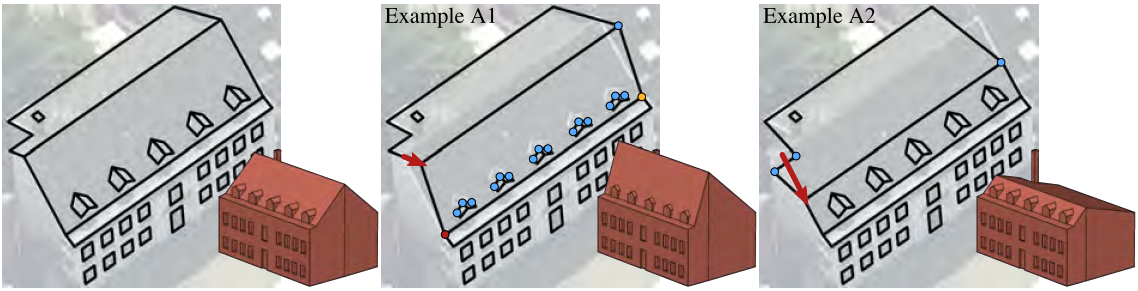
\includegraphics[width=3in]{images/modeling_L0}
  \caption{Sparse regularization: constrained modeling\cite{habbecke2012linear}. Left: original configuration. Center: editing operation such that the base plane of the dormers changes its orientation(example A1). Right: the dormers' base plane does not change(example A2). Blue vertices are relaxed in the analysis phase and automatically updated by the editing system.}
\end{figure}



%
%
%
%\cite{elhamifar2009sparse} has proposed an approach of sparse subspace clustering(SSC) considering that each data point in a union of linear subspaces can always be represented as a linear combination of the points belonging to the same linear subspace and thus the combination could be sparse if the point is written as a linear combination of all other points. This is formulated as
%
%\begin{equation}
% \label{eq:SSC}
% \min_{W}\|XW-X\|{_{F}^2}+\lambda\|W\|_{1,1},~s.t.~\textrm{diag}(W)=0
%\end{equation}
%\\
%where $X$ is represents the data points, $\|W\|_{1,1}$ is seen as a penalty item in the optimization, which favors the sparsity of the optimal solution $\overline{W}$ of which each entry measures the linear correlation between two points in the dataset. After defining the affinity matrix $S=(s_{ij})$ as $s{ij}=|\overline{w}_{ij}|+|\overline{w}_{ji}|$, the NCut method\cite{shi2000normalized} is applied to segment the object set into $K$ clusters.
%
%To reduce computation, \cite{wang2011efficient} adopts a new penalty item $\|W^{T}W\|_{1,1}$ in () as
%
%\small{
%\begin{equation}
% \label{eq:SSC}
% \begin{split}
% &\min_{W}\|XW-X\|{_{F}^2}+\lambda\|W^{T}W\|_{1,1} \\
% &s.t.~W\ge0,~\textrm{diag}(W)=0
% \end{split}
%\end{equation}
%}
%\\
%where $\|W^{T}W\|_{1,1}$ also enforces sparsity of the optimal solution $\overline{W}$.
%
%Following (), for single feature, \cite{hu2012co} gives their optimization problem
%
%\small{
%\begin{equation}
% \label{eq:SSC}
% \begin{split}
% &\min_{W_{h}}\|X_{h}W_{h}-X_{h}\|{_{F}^2}+\lambda\|W_{h}^{T}W_{h}\|_{1,1} \\
% &s.t.~W_{h}\ge0,~\textrm{diag}(W_{h})=0
% \end{split}
%\end{equation}
%}
%\\
%here $h$ corresponds to some feature descriptor, the feature matrix $X_{h}=[x_{h1},x_{h2},\cdots,x_{hN}]$ is constructed with $x_{hi}$ which is the feature vector of the $i$-th patch($i=1,2,\cdots,N$).
%
%\begin{figure}[ht]
%  \centering
%  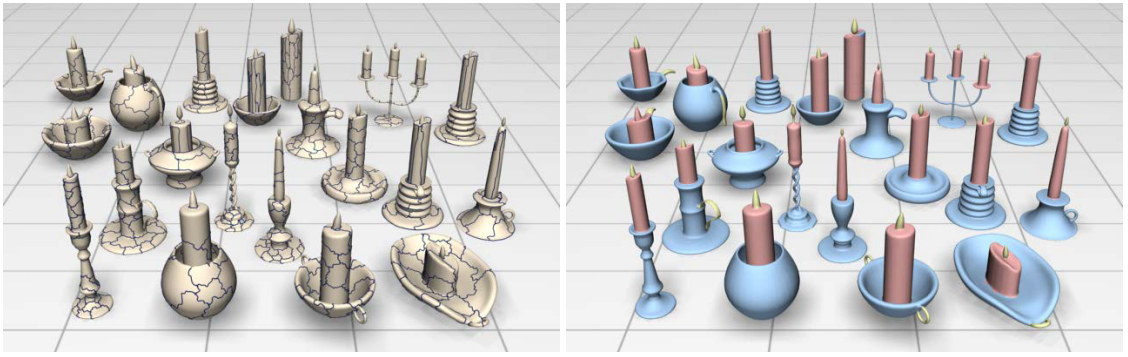
\includegraphics[width=3in]{images/co-segmentation}
%  \caption{Sparse regularization: co-segmentation\cite{hu2012co}. Left: over segmented patches. Right: co-segmented result.}
%\end{figure}
%
%





In summary, many robust point cloud consolidation or surface reconstruction techniques have been developed to deal with a variety of acquisition errors like noise, outliers, missing data(holes) or registration artifacts. Most of the $l_1$ techniques are typically too expensive to achieve interactive reconstruction times for at least moderately sized point sets, even for parallel implementations. Even though they are designed for quality rather than performance due to their nature, the performance problem is worth researching. 
\section{Dictionary Learning}
\label{sec:DictionaryLearning}

Until now, we haven't given any discussion about the overcomplete dictionary $\mathbf{D}$ that exactly leads to the sparse representations of signals.
From the definition of sparse representation, it is obvious that the choice of the dictionary will directly affect the signal processing result.

In general, this dictionary can either be chosen as a prespecified set of functions(e.g., wavelet dictionary) or designed by adapting its content to fit a given set of signal examples(e.g., \cite{aharon2006svd}).
From the performance of existing dictionary learning based works, the learned dictionaries used to outperform predefined dictionaries,
so there have been many techniques aiming to get a expressive dictionary with less computational cost.
This techniques can be directly used to deal with some geometric problem, such as compression of point cloud\cite{digne2014self}.

In this section, we also regard sparse matrix decomposition as dictionary learning.
As the name implies, sparse matrix decomposition attempts to decompose a dense matrix into the multiplication of a simple matrix(e.g., transformation matrix\cite{le2012smooth}) and the correspondent coefficient matrix which is as sparse as possible.
Generally, this decomposition is achieved with some iterative algorithm just like the dictionary learning algorithm,
so we also call the resulted simple matrix dictionary though it may not be overcomplete.

The following works show the success of dictionary learning based method in different applications.

\subsection{Linear blend skinning}

Skinning mesh animations has been an active area.
Among many proposed techniques, Linear~Blend~Skinning(LBS) is widely known to be the most popular skinning computational model due to its efficiency, simplicity, and effectiveness.
In the LBS model, skin deformation is driven by a set of bones.
Every vertex is associated with the bones via a bone-vertex weight map which quantifies the influence of each bone to the vertices.
The skin is deformed by transforming each vertex through a weighted combination of bone transformations from the rest pose.

Assume
$w_{ij}$ is the influence of $j$-th bone to the $i$-th vertex,
$p_{i}$ is the position of the $i$-th vertex at the rest pose,
$|B|$ is the number of bones, and
$R{_{j}^{t}}$ and $T{_{j}^{t}}$ are the rotation matrix and translation vector of the $j$-th bone at the $t$-th configuration, respectively,
then the deformed $i$-th vertex, $v{_{j}^{t}}$, can be computed as follows:

\small{
\begin{equation}
 \label{eq:LBS}
 v{_{j}^{t}}=\sum_{j=1}^{|B|}w_{ij}(R{_{j}^{t}}p_{i}+T{_{j}^{t}})
\end{equation}
}

By posing sparseness constraint on the weight map, the number of non-zero bone weights per vertex can be limited.
And the orthogonal constraint on $R{_{j}^{t}}$ avoids any shearing or scaling effect on the bone transformations,
thus put the transformation into rigid group.
Then the bone transformation with orthogonal rotation matrix is also called the "rigid bone".

%But the LBS model has certain limitations such as collapsing elbow and candy-wrapper effects and failure of secondary deformation.

\paragraph{(1)}
\cite{le2012smooth} introduces Smooth Skinning Decomposition with Rigid Bones(SSDR), an automated algorithm to extract the linear blending skinning, i.e., it aims to solve the inverse problem of the LBS model.

Suppose there are $|t|$ example poses of a $|V|$-vertices model, taking $\{v{_{j}^{t}}: t=1..|t|,i=1..|V|\}$ shown in () as input, SSDR decomposes them to bone transformations($R{_{j}^{t}}$, $T{_{j}^{t}}$) and the bone-vertex weight map

\small{
\begin{equation}
 \label{eq:SSDR}
 \begin{split}
 & \min_{w,R,T}E=\min_{w,R,T}\sum_{t=1}^{|t|}\sum_{i=1}^{|V|}\|v{_{j}^{t}}-\sum_{j=1}^{|B|}w_{ij}(R{_{j}^{t}}p_{i}+T{_{j}^{t}})\|^2 \\
 & s.t.~w_{ij}\ge0,~\forall i,j\\
 & ~~~~\sum_{j=1}^{|B|}w_{ij}=1,~\forall i\\
 & ~~~~|\{w_{ij}|w_{ij}\neq0\}|\le|K|,~\forall i \\
 & ~~~~{R{_{j}^{t}}}^{T}R{_{j}^{t}}=I,detR{_{j}^{t}}=1,~\forall t,j
 \end{split}
\end{equation}
}

With the sparseness constraint on the weight map, SSDR can be used for traditional skinning decomposition tasks such as animation compression and hardware-accelerated rendering.
(Figure) shows an approximation result of highly deformable model.
However, the sparseness constraint also poses certain limitations to skinning models,
e.g., it is difficult to handle exceptional vertices that are naturally associated with more than $|K|$ bones or control points.
And the relatively high computational cost makes it impractible to some degree.

\paragraph{(2)}
To address these limitations, \cite{le2013two} introduces an efficient two-layer compression technique which is formulated as a sparse dictionary learning problem. The left figure of (b) in figure..gives a clear explanation about the new technique.

Let $W\in\mathbb{R}^{k\times n}$ be the weight matrix of an input skinning model with $n$ vertices and $k$ bones, as illustrated as the top left.
At the first layer, a.k.a. $master~bone~blending$, they calculate and cache the transformations of $m$ virtual bones by blending the transformations of $k$ original bones(called $master~bones$).
At the second layer, a.k.a. $virtual~bone~blending$, they calculate the position of each vertex by blending the transformations of the virtual bones and applying the resultant transformation to the vertex.
By imposing a sparseness constraint on each blending layer, the optimization problem is formulated as

\small{
\begin{equation}
 \label{eq:TwoLayer}
 \begin{split}
 & \min_{D,A}\Delta_{W}^2=\min_{D,A}\frac{1}{kn}\|DA-W\|{_{F}^2} \\
 & s.t.~\textbf{card}(\alpha_{i})\leq2,\forall i\\
 & ~~~~~\textbf{card}(d_{i})\leq c,\forall i
 \end{split}
\end{equation}
}

By employing virtual bones to cache transformation blending of master bones,
this approach can significantly reduce computation of LBS with dense weights, with insignificant loss of accuracy of the original skinning model. Figure...
But it requires additional storage space for caching virtual bone transformations,
and transformation blending in this two-layer approach cannot go beyond certain intrinsic limitations of the LBS model,
among which sophisticated deformation effects such as muscle bulges or skin wrinkles cannot be captured well.



\vspace{15pt}
Actually, these two above methods are both not quite suitable for animation editing purposes
since their extracted bone transformations are not organized in any skeletal structures
based on which the mesh deformation is a widely-used method for animating articulated creatures such as humans and animals.
Setting up the skeleton-based animation(also known as rigging) generally consists of two main steps:
building a hierarchical skeleton with rigid bones connected by joints,
and skinning the 3D model to define how joint rotations and translations would propagate to the surface during animation.
A best result may be achieved by manually or semi-automatically repeating the two steps many times which make it costly and time-consuming.
Fortunately, the concept of using example poses can ease this problem\cite{schaefer2007example}.

\paragraph{(3)}
Attempting to take advantage of example poses, taking a set of example poses as input,
\cite{le2014ras} introduces a robust and accurate rigging framework producing its corresponding $Skeleton$-$based$ LBS model including skeletal structure, skinning weights, joint locations, and bone transformations corresponding to all the example poses.

After initializing bone transformations and determining the skeleton topology, they get the optimized LBS model by minimizing function

\small{
\begin{equation}
 \label{eq:SkeletonLBS}
 E=E_{D}+wE_{S}+\lambda E_{J}
\end{equation}
}
\\
subject to the same set of constraints () as in \cite{le2012smooth} including the \textit{sparseness~constraints}(no more than 4 non-zero weights per vertex) there and  the term $E_{D}$ is also similar to their work

\small{
\begin{equation}
 \label{eq:SRFE}
 E_{D}=\frac{1}{|t||V|}
 \sum_{t=1}^{|t|} \sum_{i=1}^{|V|}
 \|v{_{j}^{t}}
 -\sum_{j=1}^{|B|} w_{ij} ( R{_{j}^{t}}p_{i} + T{_{j}^{t}} )
 \|^2.
\end{equation}
}
\\
The term $E_{S}$ favors the smoothness of skinning weights and drives the removal of redundant bones and $E_{J}$ keeps any two connected transformations rotate around their common joint(refer to\cite{le2014ras} for the formulation).

The output can be directly used to set up skeleton-based animation in various 3D modeling and animation software as well as game engines. Despite the achieved accuracy and robustness, this approach has several limitations including the aforementioned low computational efficiency, example data dependency, and limited approximation power of the LBS model.


\begin{figure}[ht]
  \centering
  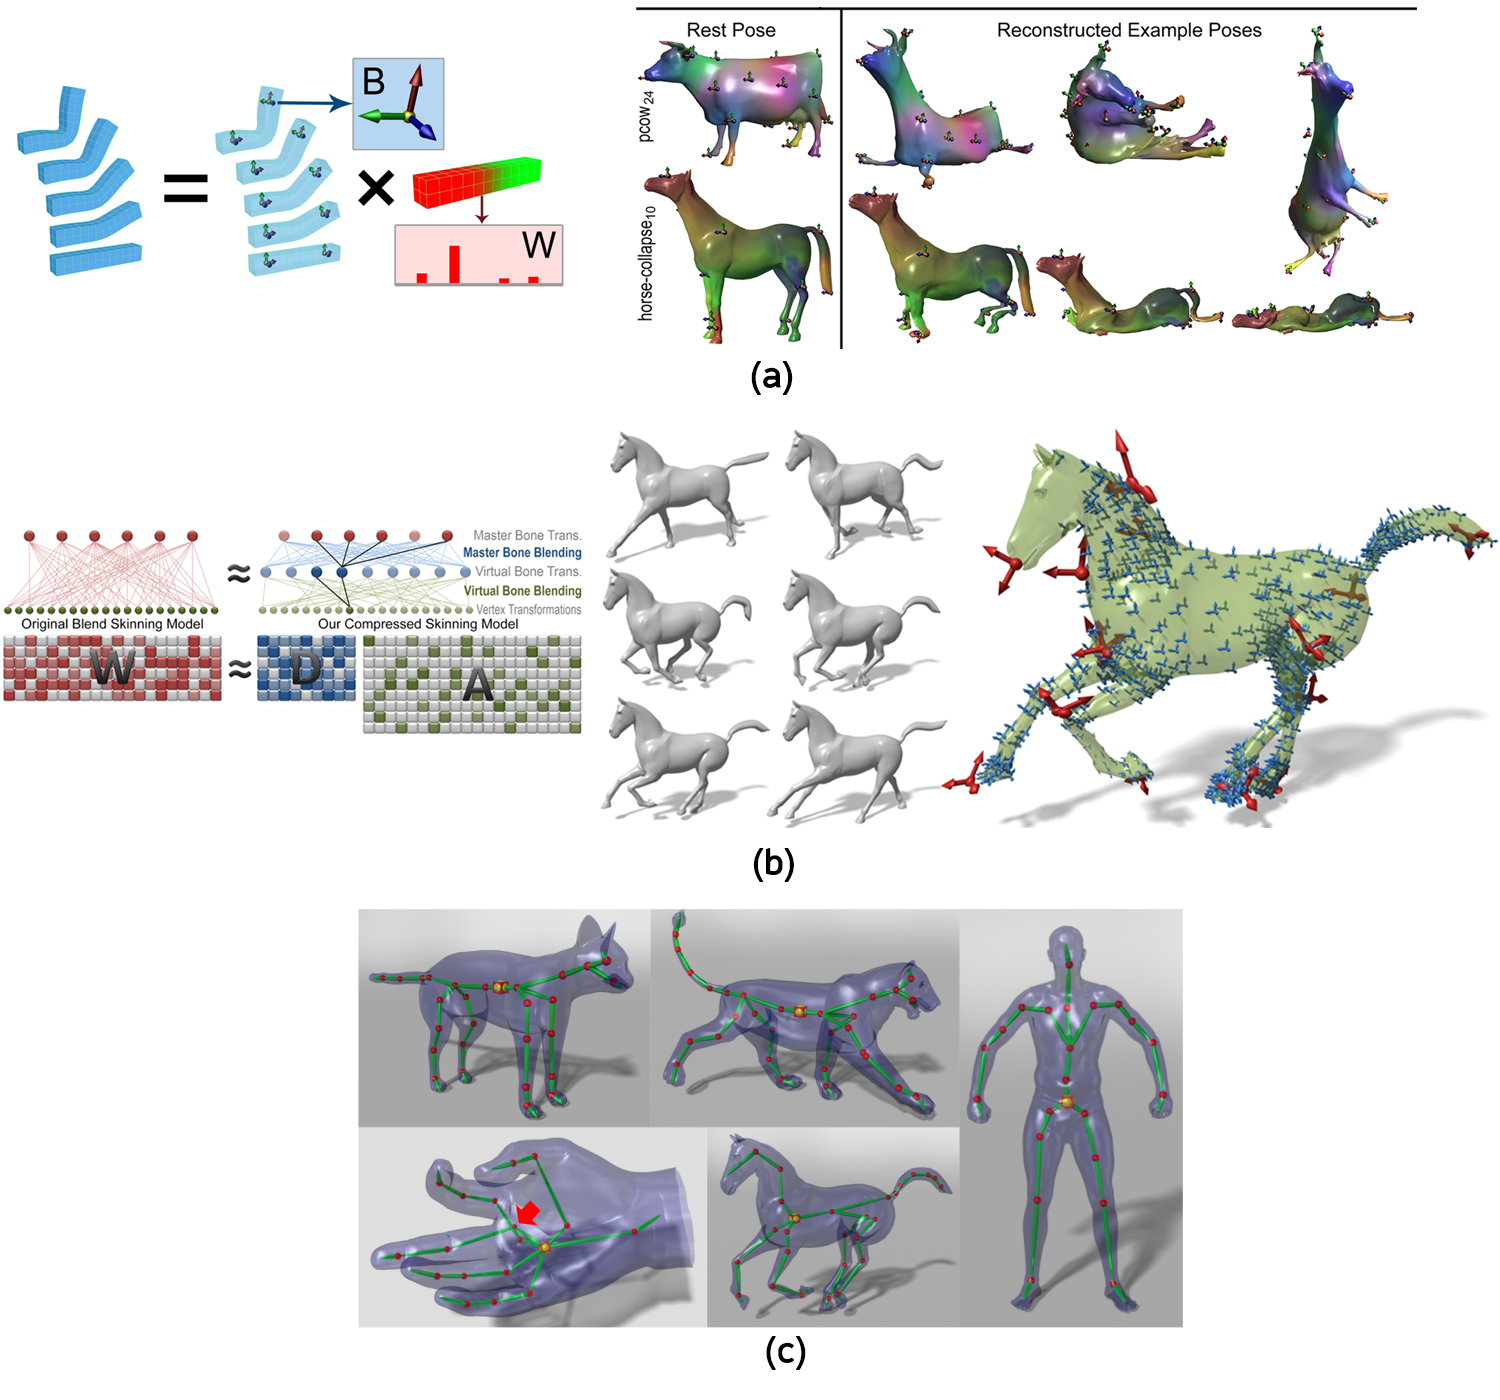
\includegraphics[width=3in]{images/skinning_decomposition}
  \caption{Dictionary learning: skinning results. (a): \cite{le2012smooth}, left: a set of example poses are decomposed into rigid bone transformation B and a sparse, convex bone-vertex weight map W. right: results of SSDR on elastic models. (b): \cite{le2013two}, left: two-layer scheme. right: an animated mesh sequence and its corresponding compressed skinning model. (c): \cite{le2014ras}, result of rigging various models such as quadrupled animals, humans, and highly deformable models.}
\end{figure}


\subsection{Deformation}

Time-varying dynamic geometry with very fine dynamic shape detail can be generated and rendered at very high visual fidelity.
When creating such content, artists usually rely on a low-dimensional control parameterization.
Despite increasing expensive power of such parameterizations and simulations, producing such realistic animations from scratch is a labor-intensive process.

As Figure.. shows, a new facial expression is generated by summing deformation components.
To decompose any mesh animations like performance faces into sparse and localized deformation modes(shown in blue),
\cite{neumann2013sparse} proposes a new efficient, easy-to-implement, and versatile data-driven approach inspired by matrix decomposition methods like sparse PCA\cite{zou2006sparse}.
Given a mesh animation with $F$ frames, each frame $f$ consists of $N$ vertices positions $\mathbf{v}{_{i}^{(f)}}$, assembling a single $'$animation matrix$'$ $\mathbf{X}\in \mathbb{R}^{F\times 3N}$ by stacking the vertices of all frames in a row-wise fashion

\small{
\begin{equation}
 \label{eq:edgecotanoperator}
 \mathbf{X} = {\left[ \begin{array}{cccc}
 (\mathbf{v}{_1^{(1)}})^{T} & (\mathbf{v}{_2^{(1)}})^{T} & \cdots & (\mathbf{v}{_{N}^{(1)}})^{T}\\
 (\mathbf{v}{_1^{(2)}})^{T} & (\mathbf{v}{_2^{(2)}})^{T} & \cdots & (\mathbf{v}{_{N}^{(2)}})^{T}\\
 \vdots & \vdots & \ddots & \vdots\\
 (\mathbf{v}{_1^{(F)}})^{T} & (\mathbf{v}{_2^{(F)}})^{T} & \cdots & (\mathbf{v}{_{N}^{(F)}})^{T}
 \end{array}
 \right]}
\end{equation}
}

After some preprocessing for $\mathbf{X}$, \cite{neumann2013sparse},
following the framework of \cite{zou2006sparse},
formulates the matrix factorization into $K$ deformation components $\mathbf{C}\in \mathbb{R}_{k\times 3N}$ with weights
$\mathbf{W}\in \mathbb{R}^{F\times K}$ as a joint regularized minimization problem

\small{
\begin{equation}
 \label{eq:sparselocal}
 \mathop{\argmin}_{\mathbf{W},\mathbf{C}}\|\mathbf{X}-\mathbf{W}\cdot\mathbf{C}\|{_{F}^2}+\Omega(\mathbf{C})~~s.t.~\mathcal{V}(\mathbf{W})
\end{equation}
}

Observing that each triplet in the rows of $\mathbf{C}$ forms a three-dimensional vector $\mathbf{c}{_{k}^{(i)}}=[x,y,z]{_{k}^{(i)}}$,
every such triplet corresponds to the x, y, and z displacement of vertex i in component k.
To make the dimensions vanish simultaneously to get \textit{sparsity}, $\Omega(\mathbf{C})$ is formulated by acting $l_1$ norm on the lengths of the displacement vectors

\small{
\begin{equation}
 \label{eq:sparselocal}
 \Omega(\mathbf{C})=\sum_{k=1}^{K}\sum_{i=1}^{N}\Lambda_{ki}\|\mathbf{c}{_{k}^{(i)}}\|_2.
\end{equation}
}
\\
The spatially-varying regularization parameters $\Lambda_{ki}$ makes it possible to enforce local support for the deformation components which is and exciting innovation.

Sparse Localized Deformation components present a versatile decomposition method for space-time mesh animation data that is applicable to many settings: editing, control, scan alignment, construction of static and parametric shape models etc.
It is mentioned in this paper that several parameters in the formulation are specified by users,
but it is not clear that whether the users should have knowledge of graphics or
whether it is easy for the users to give the suitable values.

\begin{figure}[ht]
  \centering
  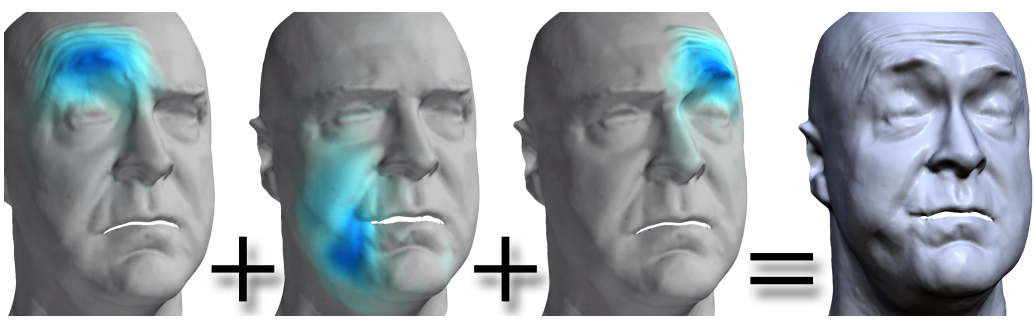
\includegraphics[width=3in]{images/localdefor_learning}
  \caption{Sparse decomposition: deformation\cite{neumann2013sparse}. A new facial expression is generated by summing deformation components, the method automatically separates spatially confined effects like separate eyebrow motions from the data.}
\end{figure}


\subsection{Reconstruction}
Surface reconstruction from point cloud is of great practical importance in computer graphics,
it takes as input a set of dense, unorganized points sampled from a subjacent, piecewise smooth surface and outputs a triangular mesh to approximate the surface.
Existing methods often realize reconstruction via a few phases with respective goals, e.g., as mentioned in section..., point cloud consolidation can be a preprocessing phasse to denoise, remove outlier and thus can reduce more reliable normal estimation.
However, integration of processing phases may not give an optimal solution.

To avoid the inherent limitations of multi-phase processing in the prior art, $\mathbf{Juyong Zhang}$ proposes a unified framework that treats geometry and connectivity construction as one joint optimization problem.

As figure..(a) shows, given a point set $\mathbb{P}=\{ \mathbf{p}_1, \mathbf{p}_2, \cdots, \mathbf{p}_n \}$(blue) sampled from a piecewise smooth surface $\textsl{S}$, 
they attempt to find a triangular mesh $\textsl{M}=\{ \mathbb{V}, \mathbb{}F\}$ with 
vertex set $\mathbb{V}=\{ \mathbf{v}_1, \mathbf{v}_2, \cdots, \mathbf{v}_m \}$(red) and triangle set $\mathbb{F}$ to approximate the underlying surface $\textsl{S}$ so that the approximation error is as small as possible

\small{
\begin{equation}
 \label{eq:dictreconstruction}
 \begin{split}
 & \min_{\mathbf{B},\mathbf{V}}\frac{1}{n}\sum_{i=1}^{n}\|\mathbf{p}_{i}-\mathbf{Vb}_{i}\|{_2^{q}}+E_{reg}\\
 & s.t.~\|b_{i}\|_0\le3,~\|b_{i}\|_1=1,~b_{i}\ge0,~\forall i \\
 & ~~~~~\mathbf{B}\in \mathbb{R}^{m\times n}
 \end{split}
\end{equation}
}
\\
where $E_{reg}$ is to regularize the reconstructed mesh to produce good mesh quality, 
each column of sparse coding matrix $\mathbf{B}$ corresponds to a triangle in mesh. Finally, all the points sampled from the region approximated by a triangle can be represented as a convex combination of the same three vertices.

Figure...shows the reconstruction result, with high triangle quality, of the Merlion model with various geometric features such as sharp and semi-sharp features and different levels of surface details. Despite these high quality results, the nonconvex optimization model makes it difficult for the solver to theoretically guarantee convergence or produce a global optimal solution. And it can fail when the point cloud has large holes or is highly non-uniform due to the current sampling method.

\begin{figure}[ht]
  \centering
  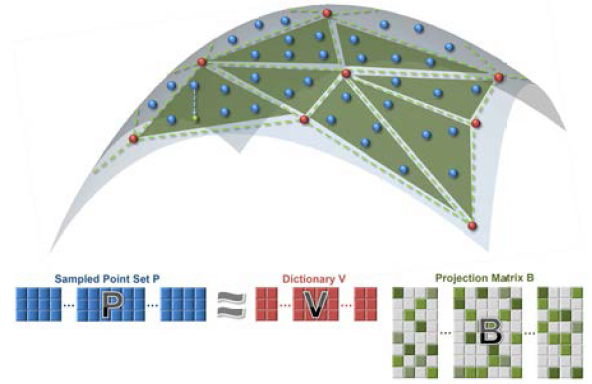
\includegraphics[width=3in]{images/reconstruction_learning}
  \caption{Dictionary learning: reconstruction\cite{}. Left: (Top)an illustration of the reconstruction problem. Given point set $\mathbb{P}$(blue) sampled from surface \textsl{S}, they approximate S with piecewise linear surface \textsl{M} with vertices $\mathbb{V}$(red) and triangles $\mathbb{F}$. (Bottom) The reconstruction problem where $\mathbf{P}$ is the position of sample point set. $\mathbf{V}$ is the dictionary and $\mathbf{B}$(green) is the sparse coding matrix that encodes triangles $\mathbb{F}$. Right: reconstruction result of the Merlion model.}
\end{figure}


\subsection{Compression}

\paragraph{(1)}The compression of unorganized point clouds have also attracted much attention due to the drastic improvement in scanner acquisition devices yielding point sets of tens of millions of points at high precision. But the counterpart of this development are datasets requiring ever higher storage capacity which results in the expensive cost in point cloud processing.

In \cite{digne2014self}, after selecting a subset of points(the seeds) that will serve as center points to cover the surface with local patches,
they compute patch descriptions using a new neighborhood descriptor((a) in Figure),
finally directly using the K-SVD algorithm \cite{aharon2006svd}

\small{
\begin{equation}
\label{eq:dictcompression}
\begin{split}
&\min_{\mathbf{D},\mathbf{X}}  \|\mathbf{Y}-\mathbf{D}\mathbf{X}\| \\
&~\mathrm{s.t.}~ \|\mathbf{x}_i\|_0 \leq s,\,\forall i
\end{split}
\end{equation}
}
\\
to exploit the self-similarity of the descriptions and build a custom dictionary $\mathbf{D}$((b) in Figure) over which all descriptors will be decomposed sparsely with $\mathbf{X}$.
Here $Y$ corresponds to the patch descriptions.
Briefly, selected patch descriptions deduce the dictionary.
Thus a new seed selection strategies or patch descriptors may result in higher performance,
this just tells the unrobustness of heuristic methods.
This compression is done at the resolution of the scanner enabling improved control of the point cloud resolution.
It achieves a filtering of noise whose magnitude is smaller than the scanner precision.
Figure(c) in Figure... gives one compression result.

\begin{figure}[ht]
  \centering
  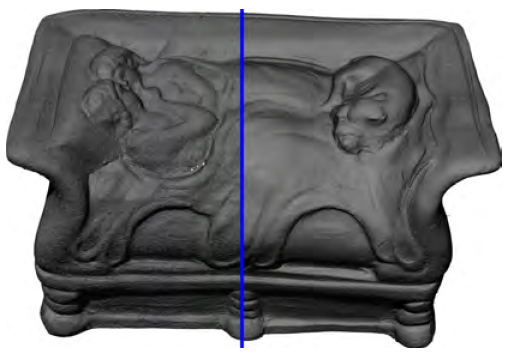
\includegraphics[width=3.0in]{images/compression_learning}
  \caption{Sparse decomposition: point cloud compression\cite{digne2014self}. (a): the local neighborhood description: a height map over a radial grid. (b): dictionary built for the Lovers(c) and the atoms are shown by order of importance(total absolute weight in the linear decompositions). (c): the Lovers(15.8 million points). By exploiting self-similarity in the model, it was compressed down to 1.15 MB. The resulting model(right) is very close to the original one(left), as the reconstruction error is less than the laser scanner precision(0.02mm) for 99.14\% of the input points.}
\end{figure}


\paragraph{(2)}
Real-time rendering of complex scenes with full global illumination is one of the main goals of computer graphics.
A popular approach is to pre-compute detailed surface light fields(SLF) describing the appearance of the objects.
However, a key problem is that an SLF data set often exhibit a very large memory footprint(often in the order of several GBs per object in the scene) and does not easily lend itself to real-time rendering.

To handle arbitrary light source configurations, general high frequency scenes and materials,
and reduce the complexity of off-line pre-computations as well as support real-time rendering,
\cite{miandji2013learning} presents a learning based algorithm for efficient compression of appearance information encoded as SLFs
which are 4D functions$f(u,v,\phi,\theta)$ represented as a \textit{hemispherical radiance distribution function}(HRDF).

After analyzing the spatial correlation in the data by clustering points with similar HRDFs,
they firstly \textit{training} a set of exemplar(basis) pairs $\{(\bar{U}_{c},\bar{V}_c)\}$ by minimizing the following energy function

\small{
\begin{equation}
 \label{eq:L1reconstruction}
 \begin{aligned}
 & E(\{\bar(U){_{a}^{c}}, \bar(V){_{a}^{c}}, \bar(S)_{ia}, M{_{ia}^{c}}\})=
   \sum_{i=1}^{} \sum_{a=1}^{}
   M{_{ia}^{c}}
   \| H{_{i}^{c}} - \bar(U){_{a}^{c}} \bar(S)_{ia} (\bar(V){_{a}^{c}})^{T}\|^2 \\
 &\mathrm{s.t.} \\
 &~~~~  (\bar(U){_{a}^{c}})^{T} \bar(U){_{a}^{c}} = (\bar(V){_{a}^{c}})^{T} \bar(V){_{a}^{c}} = I,~\forall a,\\
 &~~~~  \| \bar(S)_{ia} \|_0 \le t ~and~ \sum_{a}^{} M{_{ia}^{c}}=1,~\forall i,
 \end{aligned}
\end{equation}
}
\\
where $\bar{S}_{ia}$ contains the coefficients of the \textit{i}th HRDF when projected onto the \textit{a}th exemplar, $M$ is a binary matrix associating each HRDF to its corresponding exemplar pair$(\bar{U}{_{a}^{c}},\bar{V}{_{a}^{c}})$. Finally, let $(\xi_1, \xi_2)$ be an element of an HRDF matrix, the sparsity of $\bar{S}_i$ allows for a compact reconstruction formula for Clustered Exemplar Orthogonal Bases(CEOB)
\small{
\begin{equation}
 \label{eq:L1reconstruction}
 H{_{i}^{c}}(\xi_1, \xi_2) = \sum_{i=1}^{} \bar{U}{_{a}^{c}}(\bar{S}_{i}(t,1), \xi_1) \bar{S}_{i}(t,3) \bar(V){_{a}^{c}}(\bar{S}_{i}(t,1), \xi_2),
\end{equation}
}
\\
where $\bar{S}_{i}$ is a matrix of size $t\times3$: the first two columns describe the index of a non-zero element and the third stores its value.
Figure(b) shows three scenes with different materials.

\begin{figure}[ht]
  \centering
  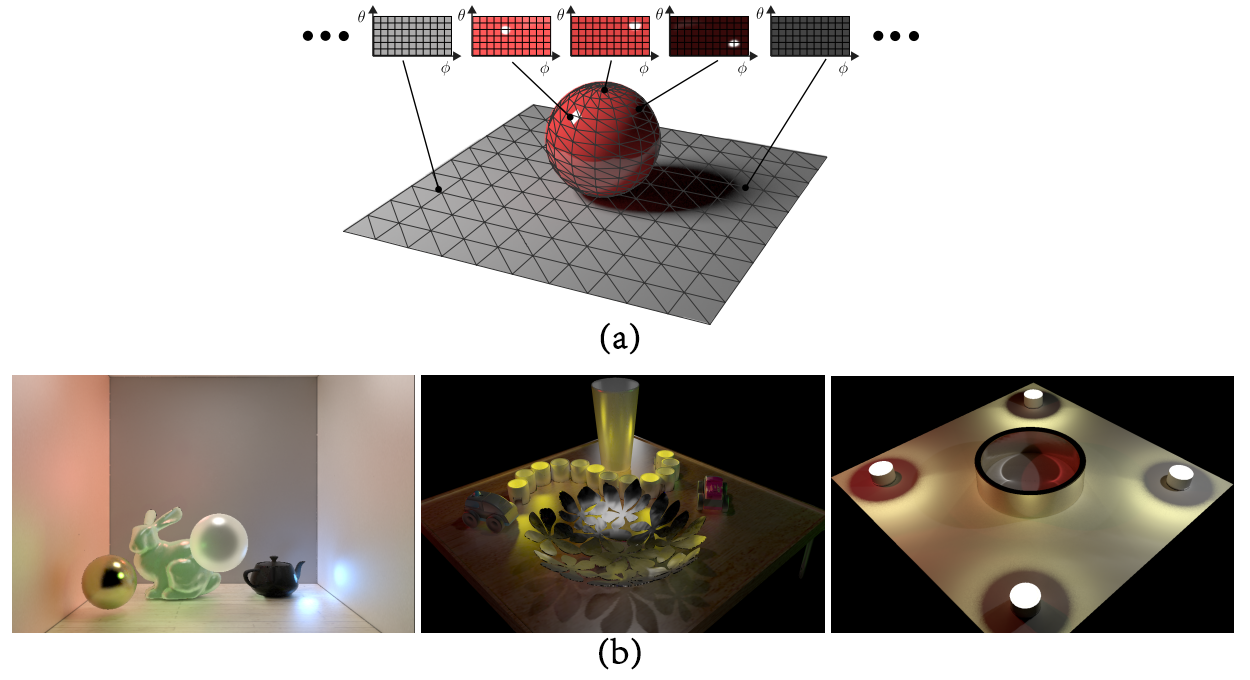
\includegraphics[width=3in]{images/rendering_learning}
  \caption{Sparse decomposition: rendering\cite{miandji2013learning}. (a): the 4D SLF function $f(u,v,\phi,\theta)$ is represented as a hemispherical radiance distribution function, HRDF. (b): rendering results using CEOB for three scenes with different materials.}
\end{figure} 
%\input{CompressedSensing}
\input{LowRank} 
\section{Acknowledgements}
\label{sec:Acknowledgements} 
\bibliography{sparsesurvey}

\end{document} 